\documentclass{siamart1116}

% basics
\usepackage[left=3cm,right=3cm,top=2.5cm,bottom=2.5cm]{geometry}
\usepackage[utf8x]{inputenc}
\usepackage[title,titletoc]{appendix}
\usepackage{afterpage}
\usepackage{enumitem}   
\setlist[enumerate]{topsep=3pt,itemsep=3pt,label=(\roman*)}

% maths
\usepackage{mathtools}
\usepackage{amsmath}
\usepackage{amssymb}
\newsiamremark{assumption}{Assumption}
\newsiamremark{remark}{Remark}
\newsiamremark{example}{Example}
\numberwithin{theorem}{section}

% tables
\usepackage{booktabs}

% plots
\usepackage{graphicx}
\usepackage{pgfplots} 
\usepackage{tikz}
\usepackage[labelfont=bf]{caption}
\setlength{\belowcaptionskip}{-5pt}
\usepackage{here}
\usepackage[font=normal]{subcaption}

% title and authors
\newcommand{\TheTitle}{A probabilistic Runge-Kutta method based on random selection of time steps for chaotic and geometric integration} 
\newcommand{\TheAuthors}{A. Abdulle, G. Garegnani}
\headers{Probabilistic Runge-Kutta method based on random time steps}{\TheAuthors}
\title{{\TheTitle}}
\author{Assyr Abdulle\thanks{Mathematics Section, \'Ecole Polytechnique F\'ed\'erale de Lausanne (\email{assyr.abdulle@epfl.ch})}
		\and
		Giacomo Garegnani\thanks{Mathematics Section, \'Ecole Polytechnique F\'ed\'erale de Lausanne (\email{giacomo.garegnani@epfl.ch})}}

% my commands 
\DeclarePairedDelimiter{\ceil}{\left\lceil}{\right\rceil}
\DeclarePairedDelimiter{\floor}{\lfloor}{\rfloor}
\DeclarePairedDelimiter{\abs}{\lvert}{\rvert}
\DeclarePairedDelimiter{\norm}{\|}{\|}
\renewcommand{\phi}{\varphi}
\renewcommand{\theta}{\vartheta}
\renewcommand{\Pr}{\mathbb{P}}
\newcommand{\eqtext}[1]{\ensuremath{\stackrel{#1}{=}}}
\newcommand{\leqtext}[1]{\ensuremath{\stackrel{#1}{\leq}}}
\newcommand{\iid}{\ensuremath{\stackrel{\text{i.i.d.}}{\sim}}}
\newcommand{\totext}[1]{\ensuremath{\stackrel{#1}{\to}}}
\newcommand{\rightarrowtext}[1]{\ensuremath{\stackrel{#1}{\longrightarrow}}}
\newcommand{\leftrightarrowtext}[1]{\ensuremath{\stackrel{#1}{\longleftrightarrow}}}
\newcommand{\pdv}[2]{\ensuremath\partial_{#2}#1}
\newcommand{\N}{\mathbb{N}}
\newcommand{\R}{\mathbb{R}}
\newcommand{\C}{\mathbb{C}}
\newcommand{\OO}{\mathcal{O}}
\newcommand{\epl}{\varepsilon}
\newcommand{\diffL}{\mathcal{L}}
\newcommand{\prior}{\mathcal{Q}}
\newcommand{\defeq}{\coloneqq}
\newcommand{\eqdef}{\eqqcolon}
\newcommand{\Var}{\operatorname{Var}}
\newcommand{\E}{\operatorname{\mathbb{E}}}
\newcommand{\MSE}{\operatorname{MSE}}
\newcommand{\trace}{\operatorname{tr}}
\newcommand{\MH}{\mathrm{MH}}
\newcommand{\ttt}{\texttt}
\newcommand{\Hell}{d_{\mathrm{Hell}}}
\newcommand{\sksum}{{\textstyle\sum}}
\newcommand{\dd}{\mathrm{d}}
\definecolor{shade}{RGB}{100, 100, 100}
\definecolor{bordeaux}{RGB}{128, 0, 50}
\newcommand{\corr}[1]{{\color{bordeaux}#1}}

\ifpdf
\hypersetup{
	pdftitle={\TheTitle},
	pdfauthor={\TheAuthors}
}
\fi

\begin{document}
	
\maketitle	

\begin{abstract} 
	We present a novel probabilistic numerical method for the integration of ODEs based on random time step selection. Theoretical analysis investigating the properties of strong and weak convergence is fully developed. We show that the measure obtained with repeated sampling converges in mean-square sense independently of the number of samples. We present the geometric properties of conservation of polynomial first integrals and symplecticity, which constitute the main advantage with respect to an additive noise method \cite{CGS16}. A complete set of numerical experiments confirms our theoretical findings.
\end{abstract}

\begin{AMS} 65L20, 65C20, 65P10 \end{AMS}

\section{Introduction} 
A variety of methods for integrating ordinary differential equations (ODEs) has been studied in the last decades. The main focus of research has been building accurate and stable deterministic approximations of the exact solution. However, these methods often provide unreliable solutions when applied to chaotic nonlinear systems of ODEs, i.e., equations for which a small perturbation in the initial condition results in a possibly large variation of the exact solution. In this case, even if the initial condition used for numerical integration is exact, which is not obtainable in floating-point precision, the deviation given by numerical errors can lead to completely wrong solutions of the underlying equation. A classic example of these problems is the Lorenz system \cite{Lor63}, a simple model of atmospheric convection, which for certain parameter values presents a typical chaotic behavior, which is nonetheless fully deterministic. Systems resulting in deterministic chaos arise in many practical applications, with the most notable example represented by chaotic chemical reactions.

In order to overcome this issue, probabilistic numerical integrators of ODEs have recently been proposed \cite{CGS16, KeH16}. These methods have the purpose of accounting for the numerical error in a statistical manner, rather than with deterministic estimates. In particular, the common underlying idea is to furnish the solution in terms of a probability distribution instead of a punctual value, as in classic solvers for ODEs. One of the most remarkable efforts is presented in Conrad et al. \cite{CGS16}, who construct probabilistic solutions with a slight modification of one-step deterministic methods, as, for example, integrators belonging to the Runge-Kutta class. In particular, they propose to perturb the deterministic numerical solution with an additive noise contribution at each time step. Scaling opportunely the noise term with respect to the time step employed for integration, they manage to explore the phase space of chaotic dynamical systems without spoiling the features of convergence of the underlying deterministic scheme. 

The main danger of adding a noise term to deterministic numerical solutions is that the random contribution can produce disruptive effects on favorable geometric features of the deterministic scheme. \corr{A direct example of this non-robust behavior is given by ODEs for which the solution is supposed to stay positive and small. In this case, the addition of a random contribution could force the solution in the negative plane, hence the numerical solution could be physically meaningless. As we mentioned above, chemical reactions are relevant problems in a probabilistic context due to their chaotic behavior. If a chemical reaction is modeled by an ODEs, then the components of the equation macroscopically describe the evolution in time of the concentration of reactants, thus it is physically incorrect to provide with negative solutions. Moreover, many of these equations present strong instabilities in case any of the components turns negative, which makes it even numerically inadvisable to have negative values. An additive noise contribution yields a non-zero probability to obtain negative solutions, which can become relevant in case the magnitude of one component is small with respect to the time step.}

Motivated by this undesirable property, we present in this work a new probabilistic method for ODEs based on a random selection of the time steps, hence turning the stochastic component of the numerical solution from additive, thus somehow artificial, to intrinsic in the scheme itself. \corr{In this way, favorable geometric properties of deterministic integrators are inherited by our probabilistic integrator. Coming back to the example of chemical reactions, a careful selection of the random variables generating the time steps prevents any trajectory of the probabilistic solver to turn negative and therefore spoil the reliability of the simulation. The development of a probabilistic integrator conserving geometric properties and which provides with robust simulations is the main contribution of this work.}

\corr{Conrad et al. show in their work that their probabilistic integrator based on additive noise converges in the strong and weak sense towards the exact solution of the original ODE, with modified convergence rates depending on the choice of the random variables. We show that similar convergence properties can be achieved with a conscious selection of the random variables producing the time steps.} In fact, setting the variance of the random time steps to be proportional to some power of a deterministic time step allows to retrieve the rates of the underlying Runge-Kutta integrator. This property is achieved and analyzed both in the strong and in the weak sense. 

It has been pointed out by Kersting and Hennig \cite{KeH16} that the performances of a probabilistic method strongly depend on the overall quality of a set of values drawn from the numerical solution. \corr{Indeed, the numerical solution given by a probabilistic integrator is a random variable, thus in order to obtain values a sampling strategy, e.g., Monte Carlo, has to be employed.} For any probabilistic solver, it is desirable that the solution converges to the exact solution when the time step tends to zero. This property is fully explained by strong and weak convergence. Following the notation introduced by Kersting and Hennig, the numerical solution is identified by a probability measure $Q_h$ which converges to the Dirac delta $\delta_y$ concentrated on the exact solution as $h\to 0$. The quantity we have access to is another measure, denoted by $Q_h(M)$, which is obtained after $M$ repeated samplings of $Q_h$. Hence, it is expected that
\begin{equation}
Q_h(M) \rightarrowtext{M\to\infty} Q_h \rightarrowtext{h\to 0} \delta_y.
\end{equation}
In this work we show that in a mean-square sense the quality of $Q_h(M)$ is independent of $M$, and therefore the computational cost due to repeated sampling can be considered as negligible. \corr{Let us remark that a similar property could be proved for the additive noise method presented by in \cite{CGS16}.}

Geometric properties of Runge-Kutta schemes have been analyzed extensively in the deterministic case \cite{HLW06}. Sufficient conditions to obtain properties such as symmetry, symplecticity and the conservation of polynomial invariants are available in literature to build optimal geometric integrator of ODEs. In case the considered ODE is Hamiltonian, employing a numerical scheme which mimics the geometric features of the exact solution yields accurate numerical approximations on the long-time. Therefore, we would like the probabilistic integrator to inherit geometric properties from its deterministic component. The method we present in this work, being only an intrinsic modification of a Runge-Kutta integrator, fully preserves all geometric properties. In particular, we show theoretically and with numerical experiments that
\begin{itemize}
	\item[-] any Runge-Kutta method with random time steps conserves linear first integrals,
	\item[-] if the Runge-Kutta method with fixed time steps conserves quadratic first integrals, then the same method with random time steps conserves quadratic first integrals,
	\item[-] if the Runge-Kutta method with fixed time steps is symplectic, then so is the same method with random time steps.
\end{itemize}
\corr{Moreover, the aforementioned robustness property of positivity of the probabilistic solution can be considered as the simplest geometric property conserved by our numerical method.} Interestingly, all the properties above are true for each trajectory of the random time-stepping integrator. We thus say that they are verified in the strong sense. For an additive noise scheme, only simplecticity is automatically inherited from the underlying deterministic scheme in the strong sense. Conversely, linear first integrals are only conserved in expectation (or weakly), while quadratic first integrals are never conserved neither in the strong nor in the weak sense. Conceiving a probabilistic integrator of ODEs which conserves all the geometric properties above for any of its realizations is the main contribution of this work.



The paper is organized as follows. In section \ref{sec:MethodIntro} we introduce the notation we will employ throughout this work and briefly present our novel numerical scheme. Then, we show in sections \ref{sec:StrongOrder} and \ref{sec:WeakOrder} the properties of strong and weak convergence of the numerical solution towards the exact solution of the ODE. In section \ref{sec:MonteCarlo} we then analyze the accuracy of Monte Carlo estimators drawn from the numerical solution. The geometric properties of the numerical scheme are presented in section \ref{sec:GeomProperties}, which we claim being the main results of this work. Finally, we show a variety of numerical experiments confirming our theoretical results in section \ref{sec:NumericalExperiments}.

\section{Method presentation}\label{sec:MethodIntro}

Let us consider a Lipschitz function $f\colon\R^d\to\R^d$ and the ODE
\begin{equation}\label{eq:ODE}
	y' = f(y), \quad y(0) = y_0 \in \R^d.
\end{equation}
In the following, we will write for simplicity the solution $y(t)$ of \eqref{eq:ODE} in terms of the flow of the ODE. In particular, we consider the family  $\{\phi_t\}_{t \geq 0}$ of functions $\phi_t\colon\R^d\to\R^d$ such that 
\begin{equation}
	y(t) = \phi_t(y_0).
\end{equation}
Given a time step $h$, let us consider a Runge-Kutta method which approximates deterministically the solution $\phi_t(y_0)$ of \eqref{eq:ODE}. In particular, we can write the numerical solution $y_k$ approximating $\phi_{t_k}(y_0)$, with $t_k = kh$ in terms of the numerical flow $\{\Psi_t\}_{t \geq 0}$, with $\Psi_t\colon\R^d\to\R^d$, which is uniquely determined by the coefficients of the method, as
\begin{equation}
	y_{k+1} = \Psi_h(y_k), \quad k = 0, 1, \ldots.
\end{equation}
In order to provide a probabilistic interpretation of the numerical solution rather than a series of punctual values, Conrad et al. propose the scheme defined by
\begin{equation}\label{eq:ProbMethAddNoise}
	Y_{k+1} = \Psi_h(Y_{k}) + \xi_k(h), \quad k = 0, 1, \ldots,
\end{equation}
where $Y_k$ is a random variable approximating $y(t_k)$ with $Y_0 = y_0$, and $\xi_k(h)$ are opportunely scaled independent and identically distributed (i.i.d.) random variables with values in $\R^d$. Maintaining the same notation as in \eqref{eq:ProbMethAddNoise}, in this work we propose instead the scheme defined by the following recurrence relation
\begin{equation}\label{eq:ProbMethVarH}
	Y_{k+1} = \Psi_{H_k}(Y_k), \quad k = 0, 1, \ldots,
\end{equation}
where $Y_k$ is still a random variable approximating $y(t_k)$ and the time steps $H_k$ are locally given by a sequence  of i.i.d. random variables with values in $\R^+$.
\begin{remark} In terms of computational cost simulating the two methods \eqref{eq:ProbMethVarH} and \eqref{eq:ProbMethAddNoise} are almost equivalent, as they imply the same number of function evaluations as the underlying deterministic solver $\Psi_h$. Nonetheless, the random time-stepping method has the slight advantage that the random variable that has to be drawn at each time step takes values in $\R^+$, while for the additive noise $\xi_k$ takes values in $\R^d$. This difference is however negligible, as modern implementations of pseudo-random generators provide with values in constant time.
\end{remark}

\section{Strong order analysis}\label{sec:StrongOrder}

The first property of \eqref{eq:ProbMethVarH} we analyze is its strong order of convergence, which gives an indication on the path-wise distance between each realization of the numerical solution and the exact solution of \eqref{eq:ODE}. Let us define the strong order of convergence. 
\begin{definition} The numerical method \eqref{eq:ProbMethVarH} has strong order $r$ for \eqref{eq:ODE} if there exists a constant $C > 0$ independent of $h$ such that
	\begin{equation}
	\E\norm{Y_k - y(kh)} \leq Ch^r
	\end{equation}
	for all $k = 1, 2, \ldots, N$.
\end{definition} 
In order to prove a result of strong convergence, we have to introduce assumptions on the random variables $\{H_k\}_{k\geq 0}$ as well as the deterministic numerical flow $\Psi_h$. Let us first consider the random time steps.
\begin{assumption}\label{as:hStrong} The i.i.d. random variables $H_k$ satisfy for all $k = 0, 1, \ldots$
	\begin{enumerate}
		\item\label{as:hStrong_Pos} $H_k > 0$ a.s.,
		\item\label{as:hStrong_E} there exists $h > 0$ such that $\E H_k = h$,
		\item\label{as:hStrong_Var} there exists $p \geq 1$ such that the scaled random variables $Z_k \defeq H_k - h$ satisfy
		\begin{equation}
			\E Z_k^2 = Ch^{2p},
		\end{equation}
		which is equivalent to $\E H_k^2 = h^2 + Ch^{2p}$.
	\end{enumerate}
\end{assumption}
The class of random variable satisfying the hypotheses above is general. However, it is practical for an implementation point of view to have examples of these variables.
\begin{example}\label{ex:uniformH} Let us consider the random variables $\{H_k\}_{k\geq 0}$ such that
	\begin{equation}
		H_k \iid \mathcal{U}(h-h^p, h+h^p), \quad 0 < h < 1, \quad p \geq 1.
	\end{equation}
	We easily verify that all the assumptions \ref{as:hStrong_Pos}, \ref{as:hStrong_E} and \ref{as:hStrong_Var} are satisfied, as 
	\begin{enumerate}
		\item $H_k > 0$ a.s. trivially since $h \leq 1$,
		\item $\E H_k = h$ since 
		\begin{equation}
			\E H_k = \frac{1}{2}(h + h^p + h - h^p) = h.
		\end{equation}
		\item The random variables $Z_k = H_k - h$ are $Z_k \sim \mathcal{U}(-h^p, h^p)$. Therefore
		\begin{equation}
			\E Z_k^2 = \frac{4h^{2p}}{12} = \frac{1}{3}h^{2p}.
		\end{equation}
	\end{enumerate}
	Another choice of random variables could simply be 
	\begin{equation}
		H_k \iid \log\mathcal{N}\big(\log h - \log\sqrt{1 + h^{2p - 2}}, \log(1 + h^{2p-2})\big),
	\end{equation}
	for which the properties above are trivially verified (with $C = 1$), provided $p > 1$.
\end{example}
The following assumption on the numerical flow is needed for proving strong convergence.
\begin{assumption}\label{as:PsiStrong} The Runge-Kutta method defined by the numerical flow $\{\Psi_t\}_{t\geq 0}$ satisfies the following properties.
	\begin{enumerate}
		\item\label{as:PsiStrong_Order} For $h$ small enough, there exists a constant $C > 0$ such that
			\begin{equation}
				\norm{\Psi_h(y) - \phi_h(y)} \leq Ch^{q+1}, \quad \forall y \in \R^d,
			\end{equation}
			\corr{i.e., the deterministic solver has order $q$.}
		\item\label{as:PsiStrong_Time} \corr{The map $t \mapsto \Psi_t(y)$ is Lipschitz continuous of constant $L_\Psi$, i.e.,}
			\begin{equation}\label{eq:LipschitzPsiT}
				\norm{\Psi_t(y) - \Psi_s(y)} \leq L_\Psi \abs{t - s}, \quad \forall t, s > 0.
			\end{equation}
		\item\label{as:PsiStrong_Space} There exists a constant $\Lambda > 0$ independent of $h$ such that 
			\begin{equation}\label{eq:LipschitzPsiY}
				\norm{\Psi_h(y) - \Psi_h(z)} \leq (1 + \Lambda h) \norm{y - z}, \quad \forall y, z \in \R^d.
			\end{equation}
	\end{enumerate}
\end{assumption}
The local strong convergence of \eqref{eq:ProbMethVarH} can now be proved. 
\begin{lemma}[Strong local order]\label{thm:StrongOrderLocal} Under Assumptions \ref{as:hStrong} and \ref{as:PsiStrong} the numerical solution $Y_1$ given by one step of \eqref{eq:ProbMethVarH} satisfies 
	\begin{equation}
	\E\norm{Y_1 - y(h)} \leq C h^{\min\{q + 1, p\}},
	\end{equation}
	where $C$ is a real positive constant independent of $h$ and the coefficients $p$, $q$ are given in the assumptions.
\end{lemma}
\begin{proof} By the triangular inequality we have for all $y \in \R^d$ 
	\begin{equation}
		\E\norm{\Psi_{H_0}(y) - \phi_h(y)} \leq \E\norm{\Psi_{H_0}(y) - \Psi_h(y)} + \E\norm{\Psi_h(y) - \phi_h(y)}.
	\end{equation}		
	We now consider Assumption \ref{as:PsiStrong}.\ref{as:PsiStrong_Time} and \ref{as:PsiStrong}.\ref{as:PsiStrong_Order}, thus getting
	\begin{equation}\label{eq:LocalErrorDecomposition}
		\E\norm{\Psi_{H_0}(y) - \phi_h(y)} \leq L_{\Psi} \E\abs{H_0 - h} + C_1 h^{q+1}.
	\end{equation}
	We now apply Jensen's inequality and Assumption \ref{as:hStrong} to obtain
	\begin{equation}
	\begin{aligned}
		\E\norm{\Psi_{H_0}(y) - \phi_h(y)} & \leq L_{\Psi} (\E\abs{H_0 - h}^{2})^{1/2} + C_1 h^{q+1}\\
		&= L_{\Psi}C_2 h^p + C_1 h^{q+1} \\
		&\leq C h^{\min\{q+1, p\}},
	\end{aligned}
	\end{equation}
	which is the desired result with $C = \max\{L_\Psi C_2, C_1\}$.
\end{proof}
As a consequence of the one-step convergence, we can prove a result of strong global convergence.
\begin{theorem}[Strong global order]\label{thm:StrongOrder} Let $t_k = kh$ for $k = 1, 2, \ldots, N$, where $Nh = T$. Then, under the assumptions of Lemma \ref{thm:StrongOrderLocal} the numerical solution given by \eqref{eq:ProbMethVarH} satisfies 
	\begin{equation}\label{eq:StrongGlobalClaim}
		\sup_{k=1,2, \ldots, N} \E\norm{Y_k - y(t_k)} \leq C h^{\min\{q, p-1/2\}},
	\end{equation}
	where $C$ is a real positive constant independent of $h$. 
\end{theorem}
\begin{proof} Let us define $e_k \defeq \E\norm{Y_k - y(t_k)}$. Thanks to the triangular inequality we have
	\begin{equation}
		e_k \leq \E\norm{\Psi_{H_{k-1}}(Y_{k-1}) - \Psi_{H_{k-1}}(y(t_{k-1}))} + \E\norm{\Psi_{H_{k-1}}(y(t_{k-1})) - \phi_{h}(y(t_{k-1}))}.
	\end{equation}
	 We then apply Assumption \ref{as:PsiStrong}.\ref{as:PsiStrong_Space} to the first term and \eqref{eq:LocalErrorDecomposition}  for the second term, thus obtaining
	\begin{equation}
		e_k \leq (1 + C_1h) e_{k - 1} + C_2 h^{q + 1} + C_3 \abs{H_{k-1} - h}.
	\end{equation}
	Hence, iterating over $k$ and noticing that $e_0 = 0$, we get
	\begin{equation}
		e_k \leq C_2 h^{q + 1} \sksum_{i=0}^{k-1} (1 + C_1h)^i + C_3 \sksum_{i=1}^{k} (1 + C_1h)^{i-1}\E\abs{H_{k-i} - h}.
	\end{equation}
	For the first term, we remark that
	\begin{equation}
	\begin{aligned}
		C_2 h^{q + 1} \sksum_{i=0}^{k-1} (1 + C_1h)^i  &\corr{\leq C_2 h^{q+1} \int_{0}^{k-1}e^{C_1 h i}\dd i} \\
			&\corr{\leq \frac{C_2}{C_1} (e^{C_1T} - 1)h^q}
	\end{aligned}
	\end{equation}
	For the second term, we have by linearity of expectation
	\begin{equation}
		C_3 \sksum_{i=1}^{k} (1 + C_1h)^{i-1}\E\abs{H_{k-i} - h} \leq C_3 e^{C_1 T} \E \sksum_{i=1}^k \abs{H_{k-i} - h}.
	\end{equation}
	We now consider the term $\E \sksum_{i=1}^k \abs{H_{k-i} - h}$. Thanks to Cauchy-Schwarz inequality and the independence of the variables $\{H_i\}_{i=0}^{k-1}$, we have
	\begin{equation}
	\begin{aligned}
		\E \sksum_{i=1}^k \abs{H_{k-i} - h} &\leq \big(\sksum_{i=1}^k \E(H_{k-i} - h)^2\big)^{1/2} \\
		&\leq \big(C_4 k h^{2p}\big)^{1/2} \\
	    &\leq (C_4T)^{1/2} h^{p - 1/2}.
	\end{aligned}
	\end{equation}
	Hence, the result is proved with \corr{$C = \max\{C_2/C_1(e^{C_1T} - 1), (C_3^2C_4T)^{1/2}e^{C_1T}\}$}.
\end{proof}

\begin{remark} Let us remark that the difference between global and local orders of convergence is not exactly one, as it usually is in the purely deterministic case. In fact, thanks to the independence of the random variables there is only a $1/2$ loss in the random part of the exponent, while the natural loss of one order is verified in the deterministic component.
\end{remark}
\begin{remark} The result of strong convergence suggests that a reasonable choice for the noise scale $p$ is to fix it to  $q + 1/2$, where $q$ is the order of the Runge-Kutta method $\Psi_h$. In this way, the properties of convergence of the underlying deterministic method are not spoiled, nonetheless getting a probabilistic interpretation of the numerical solution.
\end{remark}

\section{Weak order analysis}\label{sec:WeakOrder}

The second property we wish to analyze is the weak convergence, giving an indication of how the behavior of the numerical solution \eqref{eq:ProbMethVarH} in the mean sense. Let us define the weak order of convergence. 
\begin{definition} The numerical method \eqref{eq:ProbMethVarH} has weak order $r$ for \eqref{eq:ODE} if for any function $\Phi\in \mathcal C^\infty(\R^d, \R)$ there exists a constant $C > 0$ independent of $h$ such that
	\begin{equation}
	\abs{\E\Phi(Y_k) - \Phi(y(kh))} \leq Ch^r,
	\end{equation}
	for all $k = 1, 2, \ldots, N$.
\end{definition} 
\corr{In order to prove a result of weak convergence, we have to introduce an additional assumption on the deterministic numerical flow.
\begin{assumption}\label{as:PsiStrong_C2} The map $t \mapsto \Psi_t(y)$ is of class $\mathcal{C}^2(\R^+, \R^d)$. 
\end{assumption}}
Moreover, let us introduce the operators $\diffL$ and $\diffL^h$ such that \corr{along the trajectories of the numerical solution}
\begin{equation}
\begin{aligned}
	\Phi(\phi_h(y)) &= e^{h\diffL}\Phi(y),\\
	\E \Phi(Y_{k+1}\mid Y_k = y) &= e^{h\diffL^h}\Phi(y),
\end{aligned}
\end{equation}
for all functions $\Phi$ in $\mathcal{C}^{\infty}(\R^d, \R)$. \corr{Let us remark that the second of these relations can be addressed to as the Markov property of the probabilistic numerical solution, i.e.
\begin{equation}\label{eq:MarkovProperty}
\begin{aligned}
	\E \Phi(Y_{k}\mid Y_0 = y) &= e^{kh\diffL^h}\Phi(y)\\
		&= e^{h\diffL^h}e^{(k-1)h\diffL^h}\Phi(y)\\
		&= e^{h\diffL^h}\E \Phi(Y_{k-1}\mid Y_0 = y)
\end{aligned}
\end{equation}}
In particular, we can write explicitly $\diffL = f\cdot \nabla$, while no closed form expression for $\diffL^h$ is available. We now expand the functional of the numerical solution as follows
\begin{equation}
\begin{aligned}
	\Phi(Y_1) &= \Phi(\Psi_{H_0}(Y_0)) \\
	&= \Phi\Big(\Psi_h(Y_0) + (H_0-h)\partial_t\Psi_h(Y_0) + \frac{1}{2}(H_0-h)^2\partial_{tt}\Psi_h(Y_0) + \OO(\abs{H_0 - h}^3)\Big)\\
	&= \Phi(\Psi_h(Y_0)) + \Big((H_0 - h)\partial_t\Psi_h(Y_0)+\frac{1}{2}(H_0-h)^2\partial_{tt}\Psi_h(Y_0)\Big) \cdot \nabla\Phi(\Psi_h(Y_0))\\
	&\quad + \frac{1}{2}(H_0 - h)^2 \partial_t \Psi_h(Y_0) \partial_t \Psi_h(Y_0)^T \colon \nabla^2\Phi(\Psi_h(Y_0)) + \OO(\abs{H_0 - h}^3),
\end{aligned}
\end{equation}
where we denote by $\nabla^2\Phi$ the Hessian matrix of $\Phi$, and by $\colon$ the inner product on matrices induced by the Frobenius norm on $\R^d$, i.e., $A\colon B = \trace(A^TB)$. Taking the conditional expectation with respect to $Y_0 = y$ \corr{and applying Assumption \ref{as:hStrong}} we get
\begin{equation}
\begin{aligned}
	e^{h\diffL^h}\Phi(y) - \Phi(\Psi_h(y)) &= \frac{1}{2} Ch^{2p}\partial_{tt}\Psi_h(y)\cdot \nabla\Phi(\Psi_h(y))\\
	&\quad + \frac{1}{2} Ch^{2p}\partial_t \Psi_h(y) \partial_t \Psi_h(y)^T \colon \nabla^2\Phi(\Psi_h(y)) + \OO(h^{3p}),
\end{aligned}
\end{equation}
where we exploited Hölder inequality for the last term. Moreover, expanding $\Phi$ in $y$ we get
\begin{equation}
\begin{aligned}
	\Phi(\Psi_h(y)) &= \Phi\left(\Psi_0(y) + h\partial_t \Psi_0(y) + \OO(h^2)\right) \\
	&= \Phi(y) + \OO(h).
\end{aligned}
\end{equation}
which implies
\begin{equation}\label{eq:DistanceProbDet}
\begin{aligned}
	e^{h\diffL^h}\Phi(y) - \Phi(\Psi_h(y)) &= \frac{1}{2} Ch^{2p}\partial_{tt}\Psi_h(y) \cdot \nabla\Phi(y)\\
	&\quad +\frac{1}{2}Ch^{2p}\partial_t \Psi_h(y) \partial_t \Psi_h(y)^T \colon \nabla^2\Phi(y) + \OO(h^{2p+1}).
\end{aligned}
\end{equation}
Let us remark that thanks to Assumption \ref{as:PsiStrong}.\ref{as:PsiStrong_Order} we have
\begin{equation}\label{eq:DistanceExactDet}
	e^{h\diffL}\Phi(y) - \Phi(\Psi_h(y)) = \OO(h^{q+1}).
\end{equation}
Combining \eqref{eq:DistanceExactDet} and \eqref{eq:DistanceProbDet} we have the one-step weak error of the probabilistic method on the original ODE, i.e., 
\begin{equation}\label{eq:LocalWeakError}
	e^{h\diffL}\Phi(y) - e^{h\diffL^h}\Phi(y) = \OO(h^{\min\{2p, q+1\}}).
\end{equation}
In order to obtain a result on the global order of convergence we need a further stability assumption, which is the same as Assumption 3 in \cite{CGS16}.

\begin{assumption}\label{as:Stability} The function $f$ is in $\mathcal{C}^\infty(\R^d, \R^d)$ and all its derivatives are uniformly bounded on $\R^d$. Furthermore, $f$ is such that the operators $e^{h\diffL}$ and $e^{h\diffL^h}$ satisfy, for all functions $\Phi\in\C^{\infty}(\R^d, \R)$ and a positive constant $L$
	\begin{equation}
	\begin{aligned}
		\sup_{u\in\R^d} \abs{e^{h\diffL}\Phi(u)} &\leq (1 + Lh)\sup_{u\in\R^d}\abs{\Phi(u)},\\
		\sup_{u\in\R^d} \abs{e^{h\diffL^h}\Phi(u)} &\leq (1 + Lh)\sup_{u\in\R^d}\abs{\Phi(u)}.
	\end{aligned}
	\end{equation}
\end{assumption}

We can now state the main result on weak convergence. Let us remark that the theorem and its proof are similar to Theorem 2.4 in \cite{CGS16}.

\begin{theorem}[Weak order]\label{thm:weakOrder} Under Assumptions \ref{as:hStrong}, \ref{as:PsiStrong}, \ref{as:PsiStrong_C2} and \ref{as:Stability} there exists a constant $C > 0$ such that for all functions $\Phi\colon\R^d\to\R$ in $\mathcal{C}^\infty(\R^d,\R)$
	\begin{equation}
		\abs{\Phi(u(T)) - \E\Phi(U_N)} \leq Ch^{\min\{2p - 1, q\}},
	\end{equation}
	where $u(t)$ is the solution of \eqref{eq:ODE} and $T = Nh$. 
\end{theorem}

\begin{proof} Let us introduce the following notation
	\begin{equation}
	\begin{aligned}
		w_k &= \Phi(y(t_k) \mid y(0) = y_0)\\
		W_k &= \E\Phi(Y_k \mid Y_0 = y_0).
	\end{aligned}
	\end{equation}
	Then by the triangular inequality and the Markov property \eqref{eq:MarkovProperty} we have
	\begin{equation}
	\begin{aligned}
		\abs{w_k - W_k} \leq \abs{e^{h\diffL}w_{k-1} - e^{h\diffL^h}w_{k-1}} + \abs{e^{h\diffL^h}w_{k-1} - e^{h\diffL^h}W_{k-1}}.
	\end{aligned}
	\end{equation}
	Applying \eqref{eq:LocalWeakError} to the first term and Assumption \ref{as:Stability} to the second, we have
	\begin{equation}
		\abs{w_k - W_k} \leq Ch^{\min\{2p, q + 1\}} + (1 + Lh)\abs{w_{k-1} - W_{k-1}}.
	\end{equation} 
	Proceeding iteratively on the index $k$ and noticing that $w_0 = W_0$, we obtain
	\begin{equation}
	\begin{aligned}
		\abs{w_k - W_k} &\leq C k h^{\min\{2p, q + 1\}}\\
		&\leq C T h^{\min\{2p - 1, q\}},	
	\end{aligned}
	\end{equation}
	which is the desired result.
\end{proof}

\corr{\begin{remark} In \cite{CGS16}, Conrad et al. find ordinary and stochastic modified equations in order to prove a result of weak convergence applying techniques of backward error analysis. In particular, they show that their probabilistic solver approximates in the weak sense a stochastic differential equation (SDE) where the deterministic part is given by the original ODE. For our probabilistic solver, it is possible to prove that the numerical solutions approximates in the weak sense the solution of an SDE where the diffusion term depends on the derivative of the map $t \mapsto \Psi_t(y)$. Nonetheless, showing this result is technical and unnecessary in the scope of this work.
\end{remark}}

\section{Monte Carlo estimators}\label{sec:MonteCarlo}

The third property we analyze is the mean-square convergence of Monte Carlo estimators drawn from the random time-stepping Runge-Kutta method. Given a function $\Phi\in\mathcal{C}^\infty(\R^d, \R)$ with Lipschitz constant $L_\Phi$ and a final time $T > 0$, we consider the value $Z = \Phi(y(T))$ and its Monte Carlo estimator 
\begin{equation}\label{eq:MSE}
	\hat Z = M^{-1} \sksum_{i = 1}^M \Phi(Y_N^{(i)}),
\end{equation}
where $T = hN$ is the final time, $M$ is the number of trajectories and we denote by $\{Y_N^{(i)}\}_{i=1}^M$ a set of realizations of the numerical solution. \corr{Since we are interested in analyzing the mean square behavior of the Monte Carlo estimator, we consider its mean square error (MSE), which is defined as
\begin{equation}
	\MSE(\hat Z) = \E(Z - \hat Z)^2
\end{equation}}
Thanks to the classic decomposition of the MSE, we have
\begin{equation}\label{eq:MSEDecomposition}
	\MSE(\hat Z) = \Var \hat Z  + \big(\E(\hat Z - Z)\big)^2.
\end{equation}
Hence, applying Theorem \ref{thm:weakOrder}, we have
\begin{equation}\label{eq:MSEWeakOrder}
	\MSE(\hat Z) \leq \Var \hat Z  + Ch^{2\min\{q, 2p - 1\}}.
\end{equation}
The variance of the estimator can be trivially bounded exploiting the Lipschitz continuity of $\Phi$ and the independence of the samples by
\begin{equation}\label{eq:MSELipschitz}
\begin{aligned}
	\Var\hat Z &\leq M^{-1} L_\Phi^2 \E \norm{Y_N - y(T)}^2 \\
    &= M^{-1} L_\Phi^2 \MSE(Y_N).
\end{aligned}
\end{equation}
In order to bound the MSE of $Y_N$, defined as $\MSE(Y_N) = \E\norm{Y_N - y(T)}^2$, we apply the same decomposition of the MSE as \eqref{eq:MSEDecomposition}, which for random variables taking values in $\R^d$ reads
\begin{equation}\label{eq:MSEStrongOrder}
\begin{aligned}
	\MSE(Y_N) &= \trace(\Var Y_N) + \norm{\E\big(Y_N - y(T)\big)}^2\\
    &\leq \trace(\Var Y_N) + Ch^{\min\{2q, 2p -1\}},
\end{aligned}
\end{equation}
where we applied Jensen's inequality and Theorem \ref{thm:StrongOrder}. We can now prove a bound for the MSE of the Monte Carlo estimator.
\begin{theorem}\label{thm:MSEMonteCarlo} Under Assumptions \ref{as:hStrong} and \ref{as:PsiStrong}, the Monte Carlo estimator $\hat Z$ satisfies
	\begin{equation}
		\MSE(\hat Z) \leq C h^{\min\{2q, 2p -1\}} + \mathrm{h.o.t.},
	\end{equation}
	where $C$ is a positive constant independent of $h$.
\end{theorem}
\begin{proof} Thanks to \eqref{eq:MSEWeakOrder}, \eqref{eq:MSELipschitz} and \eqref{eq:MSEStrongOrder} we just have to show
	\begin{equation}
		\trace(\Var Y_k) \leq \hat C h^{\min\{2q, 2p - 1\}},
	\end{equation}
	for a positive constant $\hat C$ and for any $k = 1, 2, \ldots, N$. We compute a Taylor expansion of $\Psi_t(y)$ in both the $t$ and $y$ variables, thus getting
	\begin{equation}
	\begin{aligned}
		\trace(\Var Y_{k+1}) = \trace\Big(\Var\big(&\Psi_h(\E Y_k) + \partial_t \Psi_h(\E Y_k)(H_{k} - h) \\
		&+ \partial_y \Psi_h(\E Y_k)(Y_k - \E Y_k) + \OO(\abs{H_k - h}^2)\big)\Big),
	\end{aligned}
	\end{equation}
	where $\partial_y\Psi_t \in \R^{d\times d}$ is the Jacobian matrix of $\Psi_t(y)$ with respect to the $y$ variable. By independence and since all constants have null variance, we now have
	\begin{equation}
		\trace(\Var Y_{k+1}) = \trace\Big(\Var\big(\partial_t \Psi_h(\E Y_k)H_k\big)\Big) + \trace\Big(\Var\big(\partial_y \Psi_h(\E Y_k)Y_k\big)\Big) + \OO(h^{2p + 1}).
	\end{equation}
	Hence, considering Assumptions \ref{as:hStrong} and \ref{as:PsiStrong}, we get
	\begin{equation}
		\trace(\Var Y_{k+1}) \leq L_\Psi^2 \tilde Ch^{2p} + (1 + \hat C h)^2 \trace(\Var Y_k) + \OO(h^{2p + 1}).
	\end{equation}
	Denoting $v_k = \trace(\Var(Y_k))$ and since $v_0 = 0$, we can recursively bound $v_k$ as
	\begin{equation}
		v_k \leq \big(L_\Psi^2\tilde Ch^{2p} + \OO(h^{2p+1})\big) \sksum_{i=0}^{k-1}(1 + \hat C h)^2.
	\end{equation}
	\corr{Now, we bound the sum as
	\begin{equation}
		\sksum_{i=0}^{k-1}(1 + \hat Ch)^2 \leq Te^{2\hat C h}h^{-1} = Th^{-1} + 2T\hat C + \OO(h),
	\end{equation}
	thus obtaining the final inequality
	\begin{equation}
		v_k \leq TL_\Psi^2 \tilde C h^{2p - 1} + \mathrm{h.o.t.},
	\end{equation}}
	which is the desired result.
\end{proof}
\begin{remark} This result is of critical importance as it implies that the Monte Carlo estimators drawn from \eqref{eq:ProbMethVarH} converge in the mean square sense independently of the number of samples $M$ in \eqref{eq:MSE}. Hence, we can set $M = \OO(1)$ when computing Monte Carlo averages without losing accuracy in the result if $h$ is small enough. In fact, introducing as a measure of error the square root of the MSE, and imposing a fixed tolerance $\epl$, i.e.,
\begin{equation}
	\MSE(\hat Z)^{1/2} = \OO(\epl),
\end{equation}
we have thanks to Theorem \ref{thm:MSEMonteCarlo} that the time step has to satisfy
\begin{equation}
	h = \OO\big(\epl^{1 / \min\{q, p - 1/2\}}\big),
\end{equation}
regardless of the number of trajectories $M$. Therefore, the computational cost to attain such a tolerance $\epl$ is given by
\begin{equation}
	\mathrm{cost} = \OO(Mh^{-1}) = \OO(\epl^{\min\{q, p - 1/2\}}).
\end{equation}
\end{remark} 

\section{Geometric properties}\label{sec:GeomProperties}
Numerical methods for ODEs are often studied in terms of their geometric properties \cite{HLW06}. In particular, we investigate here whether the random choice of time steps in \eqref{eq:ProbMethVarH} spoils the properties of the underlying deterministic Runge-Kutta method. Let us recall the definition of first integral for an ODE.
\begin{definition} Given a function $I\colon\R^n\to\R$, then $I(y)$ is a first integral of \eqref{eq:ODE} if $I'(y)f(y) = 0$ for all $y \in \R^d$. In particular, if there exists $v \in \R^d$ such that $I(y) = v^Ty$, we say that $I$ is a linear first integral of \eqref{eq:ODE}. Moreover, if there exists a symmetric matrix $S \in \R^{d\times d}$ such that $I(y) = y^TSy$, then we say that $I$ is a quadratic first integral of \eqref{eq:ODE}.
\end{definition}
\corr{If this property of the ODE is conserved by a numerical integrator, i.e., if for the any $y\in\R^d$ it is true that $I(\Psi_h(y)) = I(y)$, then we say that the numerical method conserves the first integral. In particular, this implies that the invariant is conserved along the trajectory of the numerical solution, i.e., $I(y_k) = I(y_0)$ for all $k\geq 0$.}
	
The first issue we treat is the conservation of linear first integrals, which can be seen as a general case of the conservation of mass in physical systems.
\begin{theorem}\label{thm:LinearInvariants} The numerical method \eqref{eq:ProbMethVarH} conserves linear first integrals.
\end{theorem}
\begin{proof} For any linear first integral $I(y) = v^T y$ and by the definition of Runge-Kutta methods, we have
	\begin{equation}
		I(Y_1) = v^T y_0 + H_0 \sksum_{i=1}^s b_iv^T f(y_0 + H_0\sksum_{j=1}^{s} a_{ij}K_j),
	\end{equation}
	where $\{b_i\}_{i=1}^s$, $\{a_{ij}\}_{i,j=1}^s$ and $\{K_i\}_{i=1}^s$ are the coefficients and the internal stages of the Runge-Kutta method respectively. Since $I(y)$ is a first integral, $v^T f(y) = 0$ for any $y \in \R^d$. Hence $I(Y_1)  = I(y_0)$ \corr{and iteratively $I(Y_k) = I(y_0)$ for all $k \geq 0$ along the numerical trajectory.}
\end{proof}
\begin{remark} Let us remark that the conservation of linear first invariants is exact for any trajectory of the numerical method, and is not an average property. In other words, we can say that \eqref{eq:ProbMethVarH} conserves linear first integrals in the strong sense. For the additive noise numerical method \eqref{eq:ProbMethAddNoise}, we have
	\begin{equation}
	\begin{aligned}
		I(Y_1) &= v^T y_0 + h \sksum_{i=1}^s b_iv^T f(y_0 + h\sksum_{j=1}^{s} a_{ij}K_j) + v^T \xi_0(h), \\
		&= v^T (y_0 + \xi_0(h)).
	\end{aligned}
	\end{equation}
	If the random variable $\xi_0$ is zero-mean, then $\E I(Y_1) = I(y_0)$ and iteratively along the solution $\E I(Y_{k+1}) = \E I(Y_k) = I(y_0)$. The linear first invariants are therefore conserved in average, but not in a path-wise fashion.
\end{remark}
We now consider quadratic first invariants, which are conserved by Runge-Kutta methods that satisfy the hypotheses of Cooper's theorem \cite{HLW06}. The conservation of quadratic first invariants is of the utmost importance, e.g., for Hamiltonian systems, as it implies the symplecticity of the scheme. 
\begin{theorem}\label{thm:QuadraticInvariants} If the Runge-Kutta scheme defined by $\Psi_h$ conserves quadratic first integrals then the numerical method \eqref{eq:ProbMethVarH} conserves quadratic first integrals.
\end{theorem}
\begin{proof} Trivially, if $I(\Psi_h(y)) = I(y)$ for any $h$, then $I(\Psi_{H_0}(y)) = I(y)$ for any value that $H_0$ can assume.
\end{proof}

\begin{remark}\label{rem:QuadraticInvariants} We see from Theorem \ref{thm:QuadraticInvariants} that quadratic first integrals are conserved by each trajectory of the numerical method. Instead, for the additive noise numerical method, we find
	\begin{equation}
	\begin{aligned}
		I(Y_1) &= (\Psi_h(y_0) + \xi_0(h))^T S (\Psi_h(y_0) + \xi_0(h))^T \\
		&= I(y_0) + 2\xi_0(h)^T S  \Psi_h(y_0) + \xi_0(h)^T S \xi_0(h).
	\end{aligned}
	\end{equation}
	If the random variables are zero-mean and if there exists a matrix $Q$ such that $\E\xi_0(h)\xi_0(h)^T = Qh^{2p + 1}$ for some $p \geq 1$ (Assumption 1 in \cite{CGS16}) we then have
	\begin{equation}\label{eq:BiasQuadraticAddNoise}
		\E I(Y_1) = I(y_0) + Q h^{2p + 1} : S.
	\end{equation}
	Hence, for this method quadratic first integrals are neither conserved path-wise nor in the weak sense, as there is a bias in \eqref{eq:BiasQuadraticAddNoise}.
\end{remark}
It is known that no Runge-Kutta method can conserve any polynomial invariant of order $n \geq 3$ \cite{HLW06}. Nonetheless, for some particular problems there exist tailored Runge-Kutta methods which can conserve polynomial invariants of higher order. We therefore can state the following general result.
\begin{theorem}\label{thm:PolyInvariants} If the Runge-Kutta scheme defined by $\Psi_h$ conserves an invariant $I(y)$ for an ODE, then the numerical method \eqref{eq:ProbMethVarH} conserves $I(y)$ for the same ODE.
\end{theorem}
\begin{proof} The proof is the same as the proof of Theorem \ref{thm:QuadraticInvariants}.
\end{proof}

\subsection{Hamiltonian systems} A class of dynamical systems of particular interest for their geometric properties are the Hamiltonian systems. Given a function $E(p, q)$, called the Hamiltonian, with $p$ and $q$ in $\R^d$, they can be written as
\begin{equation}\label{eq:ODEHam}
y' = J^{-1}\nabla E(y), \quad y(0) = y_0,
\end{equation}
where the matrix $J\in\R^{2d \times 2d}$ is defined as
\begin{equation}
J = \begin{pmatrix} \mathbf{0} & I \\ -I & \mathbf{0} \end{pmatrix},
\end{equation}
and where $I$ and $\mathbf{0}$ are respectively the identity and the zero matrices in $\R^{d\times d}$. It is well-known that the flow $\phi_t\colon\R^{2d}\to\R^{2d}$ of any system of the form \eqref{eq:ODEHam} is symplectic, i.e., 
\begin{equation}\label{eq:SymplecticSystem}
\pdv{\phi_t(y)}{y}^T J \pdv{\phi_t(y)}{y} = J, \quad  
\end{equation}
where we denote by $y\in \R^{2d}$ the vector $(p, q)^T$. Condition \eqref{eq:SymplecticSystem} is equivalent in a geometric sense to saying that the flow $\phi_t$ of the system conserves areas in the phase space. In a natural manner, the flow $\Psi_h$ of a one-step numerical method for \eqref{eq:ODEHam} is called symplectic it satisfies
\begin{equation}\label{eq:SymplecticMethod}
\pdv{\Psi_h(y)}{y}^T J \pdv{\Psi_h(y)}{y} = J.
\end{equation}
It has been pointed out \cite{SkG92, HLW06} that applying an adaptive step size technique to a symplectic method can spoil the properties of simplecticity in the long-time behavior. In particular, Skeel and Gear \cite{SkG92} write any adaptive technique in function of a map $\vartheta(y, h)$ such that the $k$-th time step $h_k$ is selected as $h_k = h\vartheta(y_k, h)$, where $h$ is a base value for the time step. Hence, in order to have again a symplectic method, the new condition to be satisfied is
\begin{equation}
V^T J V = J, \quad V = \pdv{\Psi_{h\vartheta(y, h)}(y)}{y} + h\pdv{\Psi_{h\vartheta(y, h)}(y)}{h}\pdv{h\vartheta(y, h)}{y}^T.
\end{equation}
In view of this condition, we can state a result of symplecticity for our numerical scheme.
\begin{theorem}\label{thm:SymplecticRandH} If the flow $\Psi_h$ of the deterministic integrator is symplectic, then the flow of the random time-stepping probabilistic method \eqref{eq:ProbMethVarH} is symplectic.
\end{theorem}
\begin{proof} We can consider the random mapping $\vartheta(y_k, h) = \Theta_k$ such that $H_k = h\vartheta(y_k, h) = h\Theta_k$, where $\{\Theta_k\}_{k \geq 0}$ is a sequence of i.i.d. random variables such that $\Theta_k > 0$ a.s., $\E\Theta_k = 1$ and $\Var\Theta_k = h^{2p - 2}$ for any $k$ so that $H_k$ satisfies Assumption \ref{as:hStrong}. Then the probabilistic method \eqref{eq:ProbMethVarH} can be written as $Y_{k+1} = \Psi_{\Theta_k h}(Y_{k})$. Since the mapping $\vartheta(y, h)$ is independent of $y$, we have
	\begin{equation}
	V \defeq \pdv{\Psi_{\Theta_k h}(y)}{y} + h\pdv{\Psi_{\Theta_k h}(y)}{h}\pdv{\vartheta(y, h)}{y}^T = \pdv{\Psi_{\Theta_k h}(y)}{y}.
	\end{equation}
	Hence, we apply the simplecticity of the deterministic method and get
	\begin{equation}
	V^T J V = J,
	\end{equation}
	which is the desired result.
\end{proof}

Let us remark that Theorem \ref{thm:SymplecticRandH} is trivially proved from Theorem \ref{thm:QuadraticInvariants} for any deterministic method which conserves quadratic first integrals, as this property implies symplecticity for a one-step numerical method. It is though interesting that a similar reasoning can be applied to the additive noise method \eqref{eq:ProbMethAddNoise}, which does not conserve quadratic first integrals. 
\begin{theorem}\label{thm:SymplecticAddNoise} If the flow $\Psi_h$ of the deterministic integrator is symplectic, then the flow of the additive noise probabilistic method \eqref{eq:ProbMethAddNoise} is symplectic.
\end{theorem}
\begin{proof} If the flow of the deterministic integrator is $\Psi_h(y)$, the flow of the probabilistic method is given by $\tilde\Psi_h(y) = \Psi_h(y) + \xi_k(h)$. Since $\xi_k(h)$ is independent of $y$, we have $\pdv{\tilde\Psi_h(y)}{y} = \pdv{\Psi_h(y)}{y}$, which proves the result.	
\end{proof}


\section{Numerical experiments}\label{sec:NumericalExperiments}

In this section, we show numerical experiments on some classic test cases that confirm the theoretical results presented above. 

\subsection{Strong order of convergence}

\begin{table}[!t]
	\centering
	\begin{tabular}{lcccccccccc}
		\toprule
		Method & \multicolumn{5}{c}{ET} & \multicolumn{5}{c}{RK4} \\ 
		\cmidrule(l{2pt}r{2pt}){2-6} \cmidrule(l{2pt}r{2pt}){7-11} 
		$q$ & \multicolumn{5}{c}{2} & \multicolumn{5}{c}{4} \\
		$p$ & 1 & 1.5 & 2 & 2.5 & 3 & 3 & 3.5 & 4 & 4.5 & 5\\
		$\min\{q, p - 1/2\}$ & 0.5 & 1 & 1.5 & 2 & 2 & 2.5 & 3 & 3.5 & 4 & 4 \\
		strong order & 0.52 & 1.01 & 1.52 & 2.02 & 2.01 & 2.50 & 2.99 & 3.55 & 3.99 & 3.98 \\
		\bottomrule
	\end{tabular}
	\caption{Strong order of convergence for the random time-stepping explicit trapezoidal (ET) and fourth-order Runge-Kutta (RK4) as a function of the value of $p$ of Assumption \ref{as:hStrong}.}
	\label{tab:NumericalResultsStrongOrder}
\end{table}

In order to verify the strong order of convergence predicted in Theorem \ref{thm:StrongOrder}, we consider the FitzHug-Nagumo equation, which is defined as
\begin{equation}\label{eq:FitzNag}
\begin{aligned}
y_1' &= c\big(y_1 - \frac{y_1^3}{3} + y_2\big), && y_1(0) = -1, \\
y_2' &= -\frac{1}{c}(y_1 - a + by_2), && y_2(0) = 1,
\end{aligned}
\end{equation}
where $a, b, c$ are real parameters with values $a = 0.2$, $b = 0.2$, $c = 3$. We integrate the equation from time $t_0 = 0$ to final time $T = 1$. The reference solution is generated with an high order method on a fine time scale. We consider as deterministic solvers the explicit trapezoidal rule and the classic fourth order Runge-Kutta method, which verify Assumption \ref{as:PsiStrong} with $q = 2$ and $q = 4$ respectively. Moreover, we consider random time steps as in Example \ref{ex:uniformH}, where we vary $p$ in order to verify the order of convergence predicted in Theorem \ref{thm:StrongOrder}. We vary the mean time step $h$ taken by the random time steps $H_n$ in the range $h_i = 0.01^{i}$, with $i = 0, 1, \ldots, 4$. Then, we simulate $10^4$ realizations of the numerical solution $Y_{N_i}$, with $N_i = T / h_i$ for $i = 0, 1, \ldots, 4$, and compute the approximate strong order of convergence for each value of $h$ with a Monte Carlo mean. Results (Table \ref{tab:NumericalResultsStrongOrder}) show that the orders predicted theoretically by Proposition \ref{thm:StrongOrder} are confirmed numerically. 

\subsection{Weak order of convergence}

\begin{table}[t]
	\centering
	\begin{tabular}{lcccccccc}
		\toprule
		Method & \multicolumn{3}{c}{ET} & \multicolumn{5}{c}{RK4} \\ 
		\cmidrule(l{2pt}r{2pt}){2-4} \cmidrule(l{2pt}r{2pt}){5-9} 
		$q$ & \multicolumn{3}{c}{2} & \multicolumn{5}{c}{4} \\
		$p$ & 1 & 1.5 & 2 & 1 & 1.5 & 2 & 3 & 4\\
		$\min\{q, 2p - 1\}$ & 1 & 2 & 2 & 1 & 2 & 3 & 4 & 4 \\
		weak order & 0.98 & 2.06 & 2.12 & 0.90 & 1.96 & 3.01 & 3.97 & 4.08 \\
		\bottomrule
	\end{tabular}
	\caption{Weak order of convergence for the random time-stepping explicit trapezoidal (ET) and fourth-order Runge-Kutta (RK4) as a function of the value of $p$ of Assumption \ref{as:hStrong}.}
	\label{tab:NumericalResultsWeakOrder}
\end{table}

We now verify the weak order of convergence predicted in Theorem \ref{thm:weakOrder}. For this experiment we consider the ODE \eqref{eq:FitzNag} as well, with the same time scale and parameters as above. The reference solution at final time is generated in this case as well with an high-order method on a fine time scale. The deterministic integrators we choose in this experiment are the explicit trapezoidal rule and the classic fourth-order Runge-Kutta method. The mean time step varies in the range $h_i = 0.1\cdot 2^{-i}$ with $i = 0, 1, \ldots, 5$, and we vary the value of $p$ in Assumption \ref{as:hStrong} in order to verify the theoretical result of Theorem \ref{thm:weakOrder}. The function $\Phi\colon\R^d\to\R$ of the solution we consider is defined as $\phi(x) = x^Tx$. Finally, we consider $10^6$ trajectories of the numerical solution in order to approximate the expectation with a Monte Carlo sum. Results (Table \ref{tab:NumericalResultsWeakOrder}) show that the order of convergence predicted theoretically is confirmed by numerical experiments. 

\subsection{Monte Carlo estimator}

\begin{table}[t!]
	\centering
	\begin{tabular}{lcccccc}
		\toprule
		Method & \multicolumn{2}{c}{ET} & \multicolumn{4}{c}{RK4} \\ 
		\cmidrule(l{2pt}r{2pt}){2-3} \cmidrule(l{2pt}r{2pt}){4-7} 
		$q$ & \multicolumn{2}{c}{2} & \multicolumn{4}{c}{4} \\
		$p$ & 2 & 3 & 2 & 3 & 4 & 5\\
		$\min\{2q, 2p - 1\}$ & 3 & 4 & 3 & 5 & 7 & 8\\
		MSE order & 3.01 & 4.05 & 3.04 & 5.02 & 7.08 & 8.06\\
		\bottomrule
	\end{tabular}
	\caption{Convergence of the MSE of the Monte Carlo estimator for the random time-stepping explicit trapezoidal (ET) and fourth-order Runge-Kutta (RK4) with respect to $p$ of Assumption \ref{as:hStrong}.}
	\label{tab:NumericalResultsMSE}
\end{table}

In the same spirit of the previous numerical experiments, we now verify numerically the validity of Theorem \ref{thm:MSEMonteCarlo}. We consider the ODE \eqref{eq:FitzNag}, with final time $T = 10$ and the same parameters as above. In this case as well, we consider the explicit trapezoidal rule and the fourth-order explicit Runge-Kutta method with random time steps having mean $h_i = 0.1\cdot 2^{-i}$ with $i = 0, 1, \ldots, 5$. We thus vary the value of $p$ of Assumption \ref{as:hStrong} and compute the mean order of convergence over 300 repetitions of the experiment. For each repetition, we consider only one trajectory to approximate the Monte Carlo estimator, i.e., $M = 1$. We then compute the error with respect to a reference solution given by a high-order method with a small time step. Results (Table \ref{tab:NumericalResultsMSE}) show that the convergence order given in Theorem \ref{thm:MSEMonteCarlo} is respected in practice.

\subsection{Robustness} In this numerical experiment we verify the robustness of the random time-stepping probabilistic method \eqref{eq:ProbMethVarH} when applied to chemical reactions. Let us consider the Peroxide-Oxide chemical reaction, which is macroscopically defined the following balance equation
\begin{equation}
	\mathrm{O}_2 + 2\mathrm{NADH} + 2\mathrm{H}^+ \to 2\mathrm{H}_2\mathrm{O} + 2\mathrm{NAD}^+.
\end{equation}
This reaction has to be catalyzed by an enzyme to take place, which reacts with the reagents to create intermediate products of the reaction. A successful model \cite{Ols83} to describe the time-evolution of the chemical system is the following
\begin{equation}
\begin{aligned}
	\mathrm{B} + \mathrm{X} &\rightarrowtext{k_1} 2 \mathrm{X}, 
	&&2\mathrm{X} \rightarrowtext{k_2} 2\mathrm{Y}, 
	&&\mathrm{A} + \mathrm{B} + \mathrm{Y} \rightarrowtext{k_3} 3 \mathrm{X}, \\
	\mathrm{X} &\rightarrowtext{k_4} \mathrm{P}, 
	&&\mathrm{Y} \rightarrowtext{k_5} \mathrm{Q}, 
	&&\mathrm{X_0} \rightarrowtext{k_6} \mathrm{X}, \\
	\mathrm{A_0} &\leftrightarrowtext{k_7} \mathrm{A}, 
	&&\mathrm{B_0} \rightarrowtext{k_8} \mathrm{B}.
\end{aligned}
\end{equation}
Here, A and B are respectively $[\mathrm{O}_2]$ and $[\mathrm{NADH}]$, P, Q are the products and X, Y are intermediates results of the reaction process. It is therefore possible to model the time evolution of the reaction with the following system of nonlinear ODEs 
\begin{equation}\label{eq:PeroxOx}
\begin{aligned}
	\mathrm{A}' &= k_7  (\mathrm{A}_0 - \mathrm{A}) - k_3  \mathrm{A}\mathrm{B}\mathrm{Y}, &&\mathrm{A}(0) = 6, \\
	\mathrm{B}' &= k_8\mathrm{B}_0 - k_1  \mathrm{B}\mathrm{X} - k_3  \mathrm{A}\mathrm{B}\mathrm{Y}, &&\mathrm{B}(0) = 58, \\
	\mathrm{X}' &= k_1  \mathrm{B}\mathrm{X} - 2  k_2  \mathrm{X}^2 + 3  k_3 \mathrm{A}\mathrm{B}\mathrm{Y} - k_4  \mathrm{X} + k_6\mathrm{X}_0,&& \mathrm{X}(0) = 0, \\
	\mathrm{Y}' &= 2  k_2  \mathrm{X}^2 - k_5  \mathrm{Y} - k_3  \mathrm{A}\mathrm{B}\mathrm{Y}, && Y(0) = 0,
\end{aligned}
\end{equation}
where $\mathrm{A}_0 = 8$, $\mathrm{B}_0 = 1$, $\mathrm{X}_0 = 1$ and the real parameters $k_i$, $i = 1, \ldots, 8$ representing the reaction rates take values
\begin{equation}
\begin{aligned}
k_1 &= 0.35, &&k_2 = 250, &&k_3 = 0.035, &&k_4 = 20,\\
k_5 &= 5.35, &&k_6 = 10^{-5}, &&k_7 = 0.1, &&k_8 = 0.825.
\end{aligned}
\end{equation}            
It has been shown \cite{Ols83} that for these values of the parameters the system exhibits a chaotic behavior. In particular, at long time the trajectories are captured in a strange attractor, and the system shows a strong sensitivity to perturbations on the initial condition. 

Since the components of the solution represent the concentration of chemicals, we require the numerical solution to be positive. Apart from physical considerations, numerically we observe that if one of the components takes negative values, the solution shows strong instabilities. Let us consider the maximum time step $h_{\max}$ for which the deterministic numerical solution stays positive and thus is stable. The probability that the probabilistic method presents instabilities before a time $T = hN$ is therefore given by
\begin{equation}
	\Pr(Y_k \text{ is unstable}) = \Pr\big(\textstyle \bigcup_{k=1}^N A_k\big), \quad A_k = \{H_k > h_{\max}\}.
\end{equation}
Depending on the distribution of the variables $H_k$, this probability can be computable explicitly. If they are drawn from a uniform distribution as in Example \ref{ex:uniformH}, we can just set $h + h^p < h_{\max}$ thus having a null probability of being unstable. Conversely, for the additive noise method we can have disruptive effects even with small time steps if the solution has a small magnitude. Let us consider a one-dimensional problem and \eqref{eq:ProbMethAddNoise} with $\xi_k(h)$ i.i.d. random variables $\mathcal{N}(0, h^{2p + 1})$. Then, for example, if the deterministic method would predict from time $t_k = kh$ to time $t_{k+1}$ a value $\Psi_h(Y_k) = h^{p + 1/2}$, the probability that $Y_{k+1}$ is negative is
\begin{equation}
	\Pr(Y_{k+1} < 0 \mid \Psi_h(Y_k) = h^p) = \frac{1}{2}(1 + \mathrm{erf}(-1 / \sqrt{2})) \approx 0.16.
\end{equation}
Hence, integrating over long time an equation whose components should stay positive with a small magnitude employing the additive noise method likely produces instabilities regardless of the chosen time step.

Let us apply the additive noise method \eqref{eq:ProbMethAddNoise} and the random time-stepping scheme \eqref{eq:ProbMethVarH} to equation \eqref{eq:PeroxOx}. We choose $h = 0.05$ as the mean time steps for \eqref{eq:ProbMethVarH} and as the time step for \eqref{eq:ProbMethAddNoise}, while we employ the stabilized explicit Runge-Kutta-Chebyshev method (RKC) \cite{HoK71} as deterministic integrator. Results (Figure \ref{fig:OxPeroxTraj}) show that the method we propose in this work conserves the positivity of the numerical solution while capturing the chaotic nature of the chemical reaction, while the additive noise scheme produces negative values, thus showing strong instabilities in the long-time behavior.
\begin{figure}
	\begin{center} 
		\begin{subfigure}[b]{1\textwidth}
			\centering
			\hspace{-0.3cm}\includegraphics[]{OxPerox}
		\end{subfigure}	
		\begin{subfigure}[b]{1\textwidth}
			\centering
			\includegraphics[]{OxPeroxAdd}
		\end{subfigure} 
	\end{center}
	\caption{Thirty trajectories of the numerical value of the concentration of the X species for the random time-stepping and additive noise methods.}
	\label{fig:OxPeroxTraj}
\end{figure}

\subsection{Conservation of quadratic first integrals} 

\begin{figure}[t]
	\begin{center}
		\begin{tabular}{c@{\hspace{0.3cm}}c}
			\includegraphics[]{KeplerOne} & \includegraphics[]{KeplerTwo} \\
			\includegraphics[]{KeplerOneAdd} & \includegraphics[]{KeplerTwoAdd} \\
		\end{tabular}
	\end{center}
	\hspace{0.84cm}\includegraphics[]{KeplerMom}
	\caption{Trajectories of \eqref{eq:KeplerPert} given by \eqref{eq:ProbMethVarH} for $0 \leq t \leq 200$ and $3800 \leq t \leq 4000$ (first row, left and right), and by \eqref{eq:ProbMethAddNoise} for $0 \leq t \leq 200$ and $200 \leq t \leq 400$ (second row, left and right). Error on the angular momentum for $0 \leq t \leq 4000$ given by the two methods.}
	\label{fig:Kepler}
\end{figure}

We consider the Kepler system with perturbation, a simple model for the two-body problems in celestial mechanics, which reads
\begin{equation}\label{eq:KeplerPert}
\begin{aligned}
	q_1' &= p_1, && p_1' = -\frac{q_1}{\norm{q}^3} - \frac{\delta q_1}{\norm{q}^5}, \\
	q_2' &= p_2, && p_2' = -\frac{q_2}{\norm{q}^3} - \frac{\delta q_2}{\norm{q}^5},
\end{aligned}
\end{equation}
where $p_1$, $p_2$ are the two components of the velocity and $q_1$, $q_2$ are the two components of the position. We assume the perturbation parameter $\delta$ to be equal to 0.015 and the initial condition to be
\begin{equation}
	q_1(0) = 1 − e,\quad q_2(0) = 0, \quad p_1(0) = 0, \quad p_2(0) = \sqrt{(1 + e)/(1 − e)},
\end{equation}
where $e = 0.6$ is the eccentricity. It is well-known that this equation has the Hamiltonian and the angular momentum as quadratic first integrals. In particular, we focus here on the angular momentum, which reads
\begin{equation}
	I(p, q) = q_1p_2 - q_2p_1.
\end{equation}
We consider the simplest Gauss collocation method, the implicit midpoint rule, as the deterministic Runge-Kutta method. It is known that all the integrators based on Gauss nodes conserve quadratic first integrals. We expect therefore that the random time-stepping method \eqref{eq:ProbMethVarH} implemented with $\Psi_h$ given by the implicit midpoint rule conserves this property thanks to Theorem \ref{thm:QuadraticInvariants}. We therefore integrate \eqref{eq:KeplerPert} with mean time step $h = 0.01$ from time $t = 0$ to time $t = 4000$ which corresponds to approximately $636$ revolutions of the system, thus considering the long-time behavior of the numerical solution. Moreover, we consider the additive noise method \eqref{eq:ProbMethAddNoise} with $h = 0.01$, expecting that the first integral will not be conserved. Results (Figure \ref{fig:Kepler}) show that the method \eqref{eq:ProbMethVarH} conserves perfectly the angular momentum, while \eqref{eq:ProbMethAddNoise} satisfies the result shown in Remark \ref{rem:QuadraticInvariants} only in the short time, while in the long time the solution does not reflect the physical features of the underlying system.

\subsection{Chaotic Hamiltonian systems}

\begin{figure}[t!]
	\begin{center}
		\begin{tabular}{c@{\hspace{0.3cm}}c}
			\includegraphics[]{HHStep} & \includegraphics[]{HHAdd} \\
		\end{tabular}
	\end{center}
	\begin{tabular}{l}
		\hspace{0.72cm}\includegraphics[]{HHStepChaos} \\
		\hspace{0.5cm}\includegraphics[]{HHStepHam}
	\end{tabular}
	\caption{A trajectory of \eqref{eq:HenHei} given by \eqref{eq:ProbMethVarH} for $0 \leq t \leq 350$ (first row, left), and by \eqref{eq:ProbMethAddNoise} (first row, right). Value of $q_1$ for the whole set of realizations of \eqref{eq:ProbMethVarH} for $0 \leq t \leq 600$. Error on the Hamiltonian for $0 \leq t \leq 600$.}
	\label{fig:HH}
\end{figure}

Probabilistic methods for differential equations are of particular interest when applied to chaotic systems. Hamiltonian systems can present chaotic features in the long-time behavior, while conserving geometric properties. It is therefore relevant to study whether both the geometric features and the chaotic nature are captured by the probabilistic integrator. An example of this class of system is given by the Hénon-Heiles problem \cite{HeH64}, whose Hamiltonian is given by
\begin{equation}\label{eq:HenHeiHam}
	H(p, q) = \frac{1}{2}\norm{p}^2 + \frac{1}{2}\norm{q}^2 + q_1^2q_2 - \frac{1}{3}q_2^3,
\end{equation}
where $p$ and $q$ are vectors of $\R^2$ representing velocity and position respectively. The corresponding system of ODEs can then be written as
\begin{equation}\label{eq:HenHei}
\begin{aligned}
	p' &= -\nabla_q H(p, q), &&p(0) = p_0 \in \R^2,\\
	q' &= \nabla_p H(p, q), &&q(0) = q_0 \in \R^2.
\end{aligned}
\end{equation}
It is well-known that this systems presents typical deterministic chaos for values $H > 1/8$. We consider as the deterministic integrator the $s$-stage trapezoidal rule \cite{IaT09}, which is defined by its coefficients $\{b_i\}_{i=1}^s$, $\{c_i\}_{i=1}^s$, with $c_1 = 0$ and $c_s = 1$. The coefficients $\{a_{ij}\}_{i,j=1}^s$ are then determined as $a_{ij} = c_ib_j$. It has been proved that this numerical scheme conserves polynomial Hamiltonians of degree less than $s$ for $s$ even, or $s + 1$ for $s$ odd. Thanks to Theorem \ref{thm:PolyInvariants}, if we choose as the $s$-stage trapezoidal rule, with $s \geq 4$, as the deterministic component $\Psi_h$ of \eqref{eq:ProbMethVarH}, the Hamiltonian \eqref{eq:HenHeiHam} should be conserved exactly by all the numerical trajectories. On the other hand, we do not expect the additive noise method \eqref{eq:ProbMethAddNoise} to conserve the Hamiltonian in this case.

For this numerical experiment, we assume the initial condition to be
\begin{equation}
	q_1(0) = 0.5,\quad q_2(0) = 0, \quad p_1(0) = 0, \quad p_2(0) = 0.1,
\end{equation}
so that the Hamiltonian is $H = 0.13 > 1/8$ and \eqref{eq:HenHei} is in the chaotic regime. We then integrate the equation for time $t \in [0, 600]$ with the two probabilistic versions of the five-stage trapezoidal rule choosing as mean time step $h = 0.01$ for \eqref{eq:ProbMethVarH} and fixing $h = 0.01$ for \eqref{eq:ProbMethAddNoise}. We compute $M = 10$ trajectories for both the numerical methods. Results (Figure \ref{fig:HH}) show that each trajectory given by the random time-stepping technique conserves the Hamiltonian function, nonetheless capturing the chaotic behavior of the system at long time. In fact, after a short time where all trajectories approximately coincide, the attractor in the phase space is explored fully by the set of trajectories. On the other hand, the additive noise method does not conserve the Hamiltonian neither path-wise nor in the mean sense. Furthermore, due to this deviation from the correct energy value, all trajectories present an unstable behavior after a short time, while the random time-stepping technique is stable for the same value of $h$.

\subsection{Bayesian inferential problems} 

\begin{figure}[t!]
	\begin{center}
		\begin{tabular}{c@{\hspace{0.1cm}}c}
			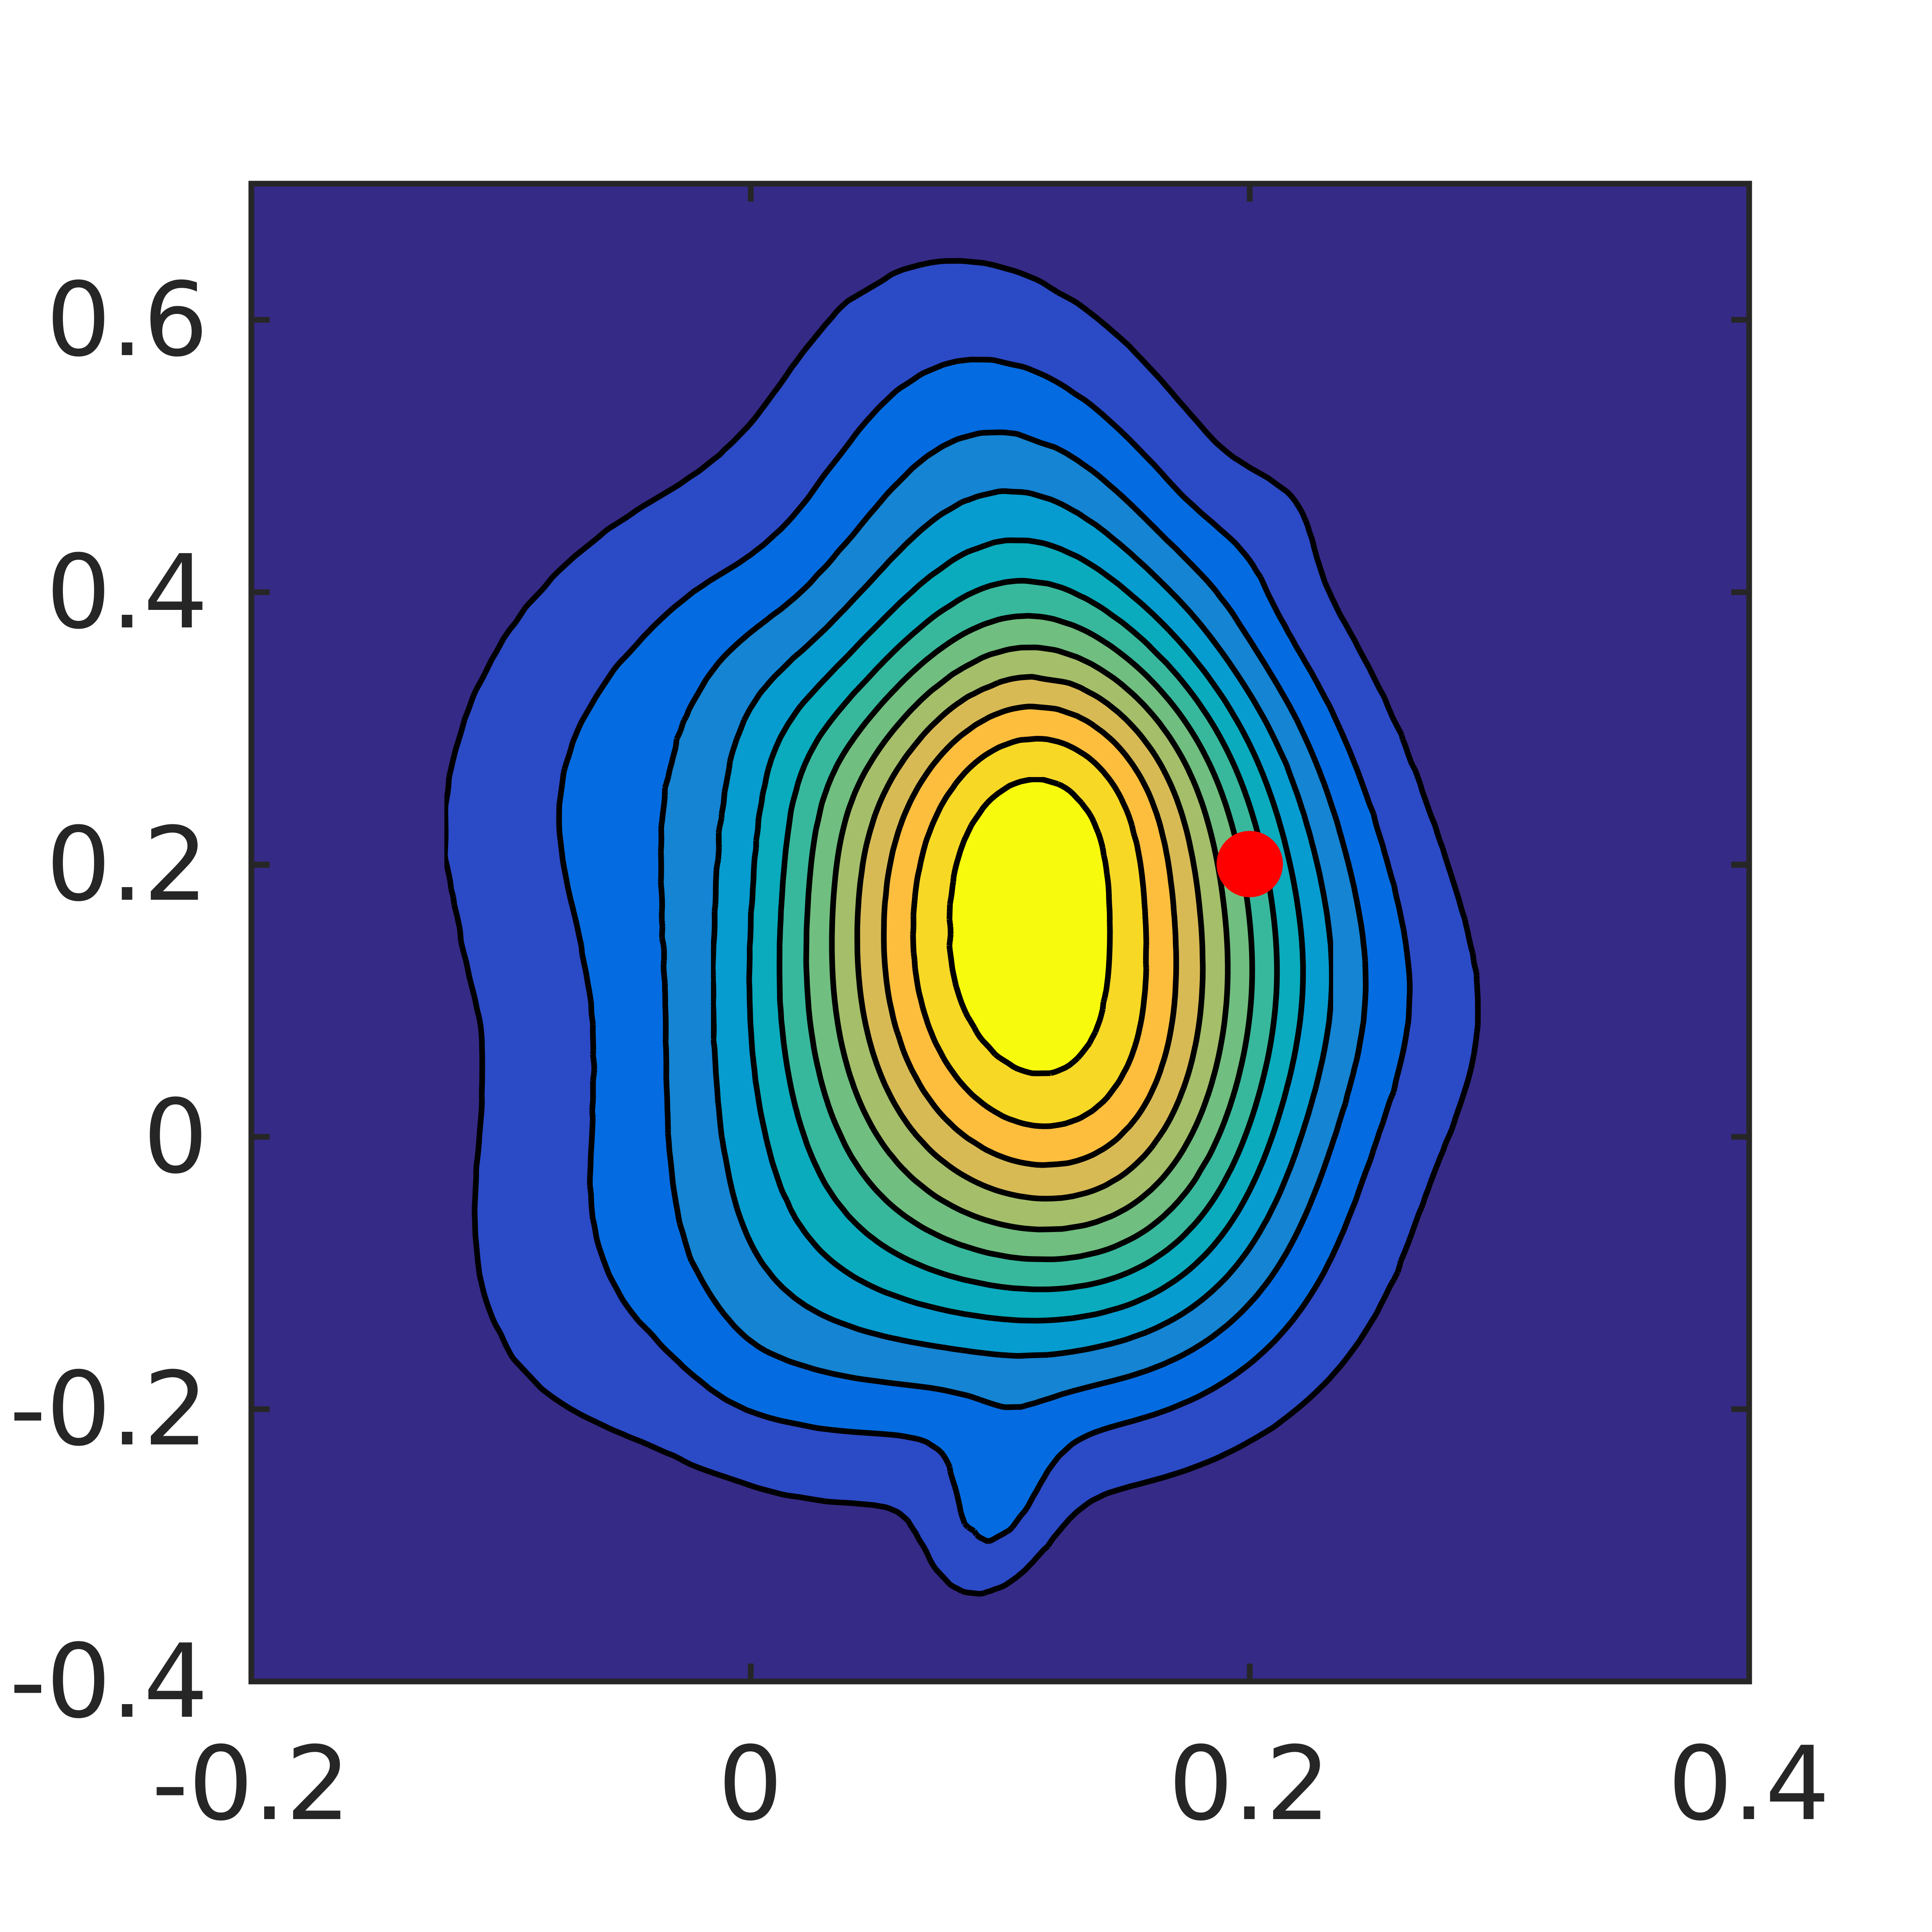
\includegraphics[]{MCMCFitznagStep01.png} & 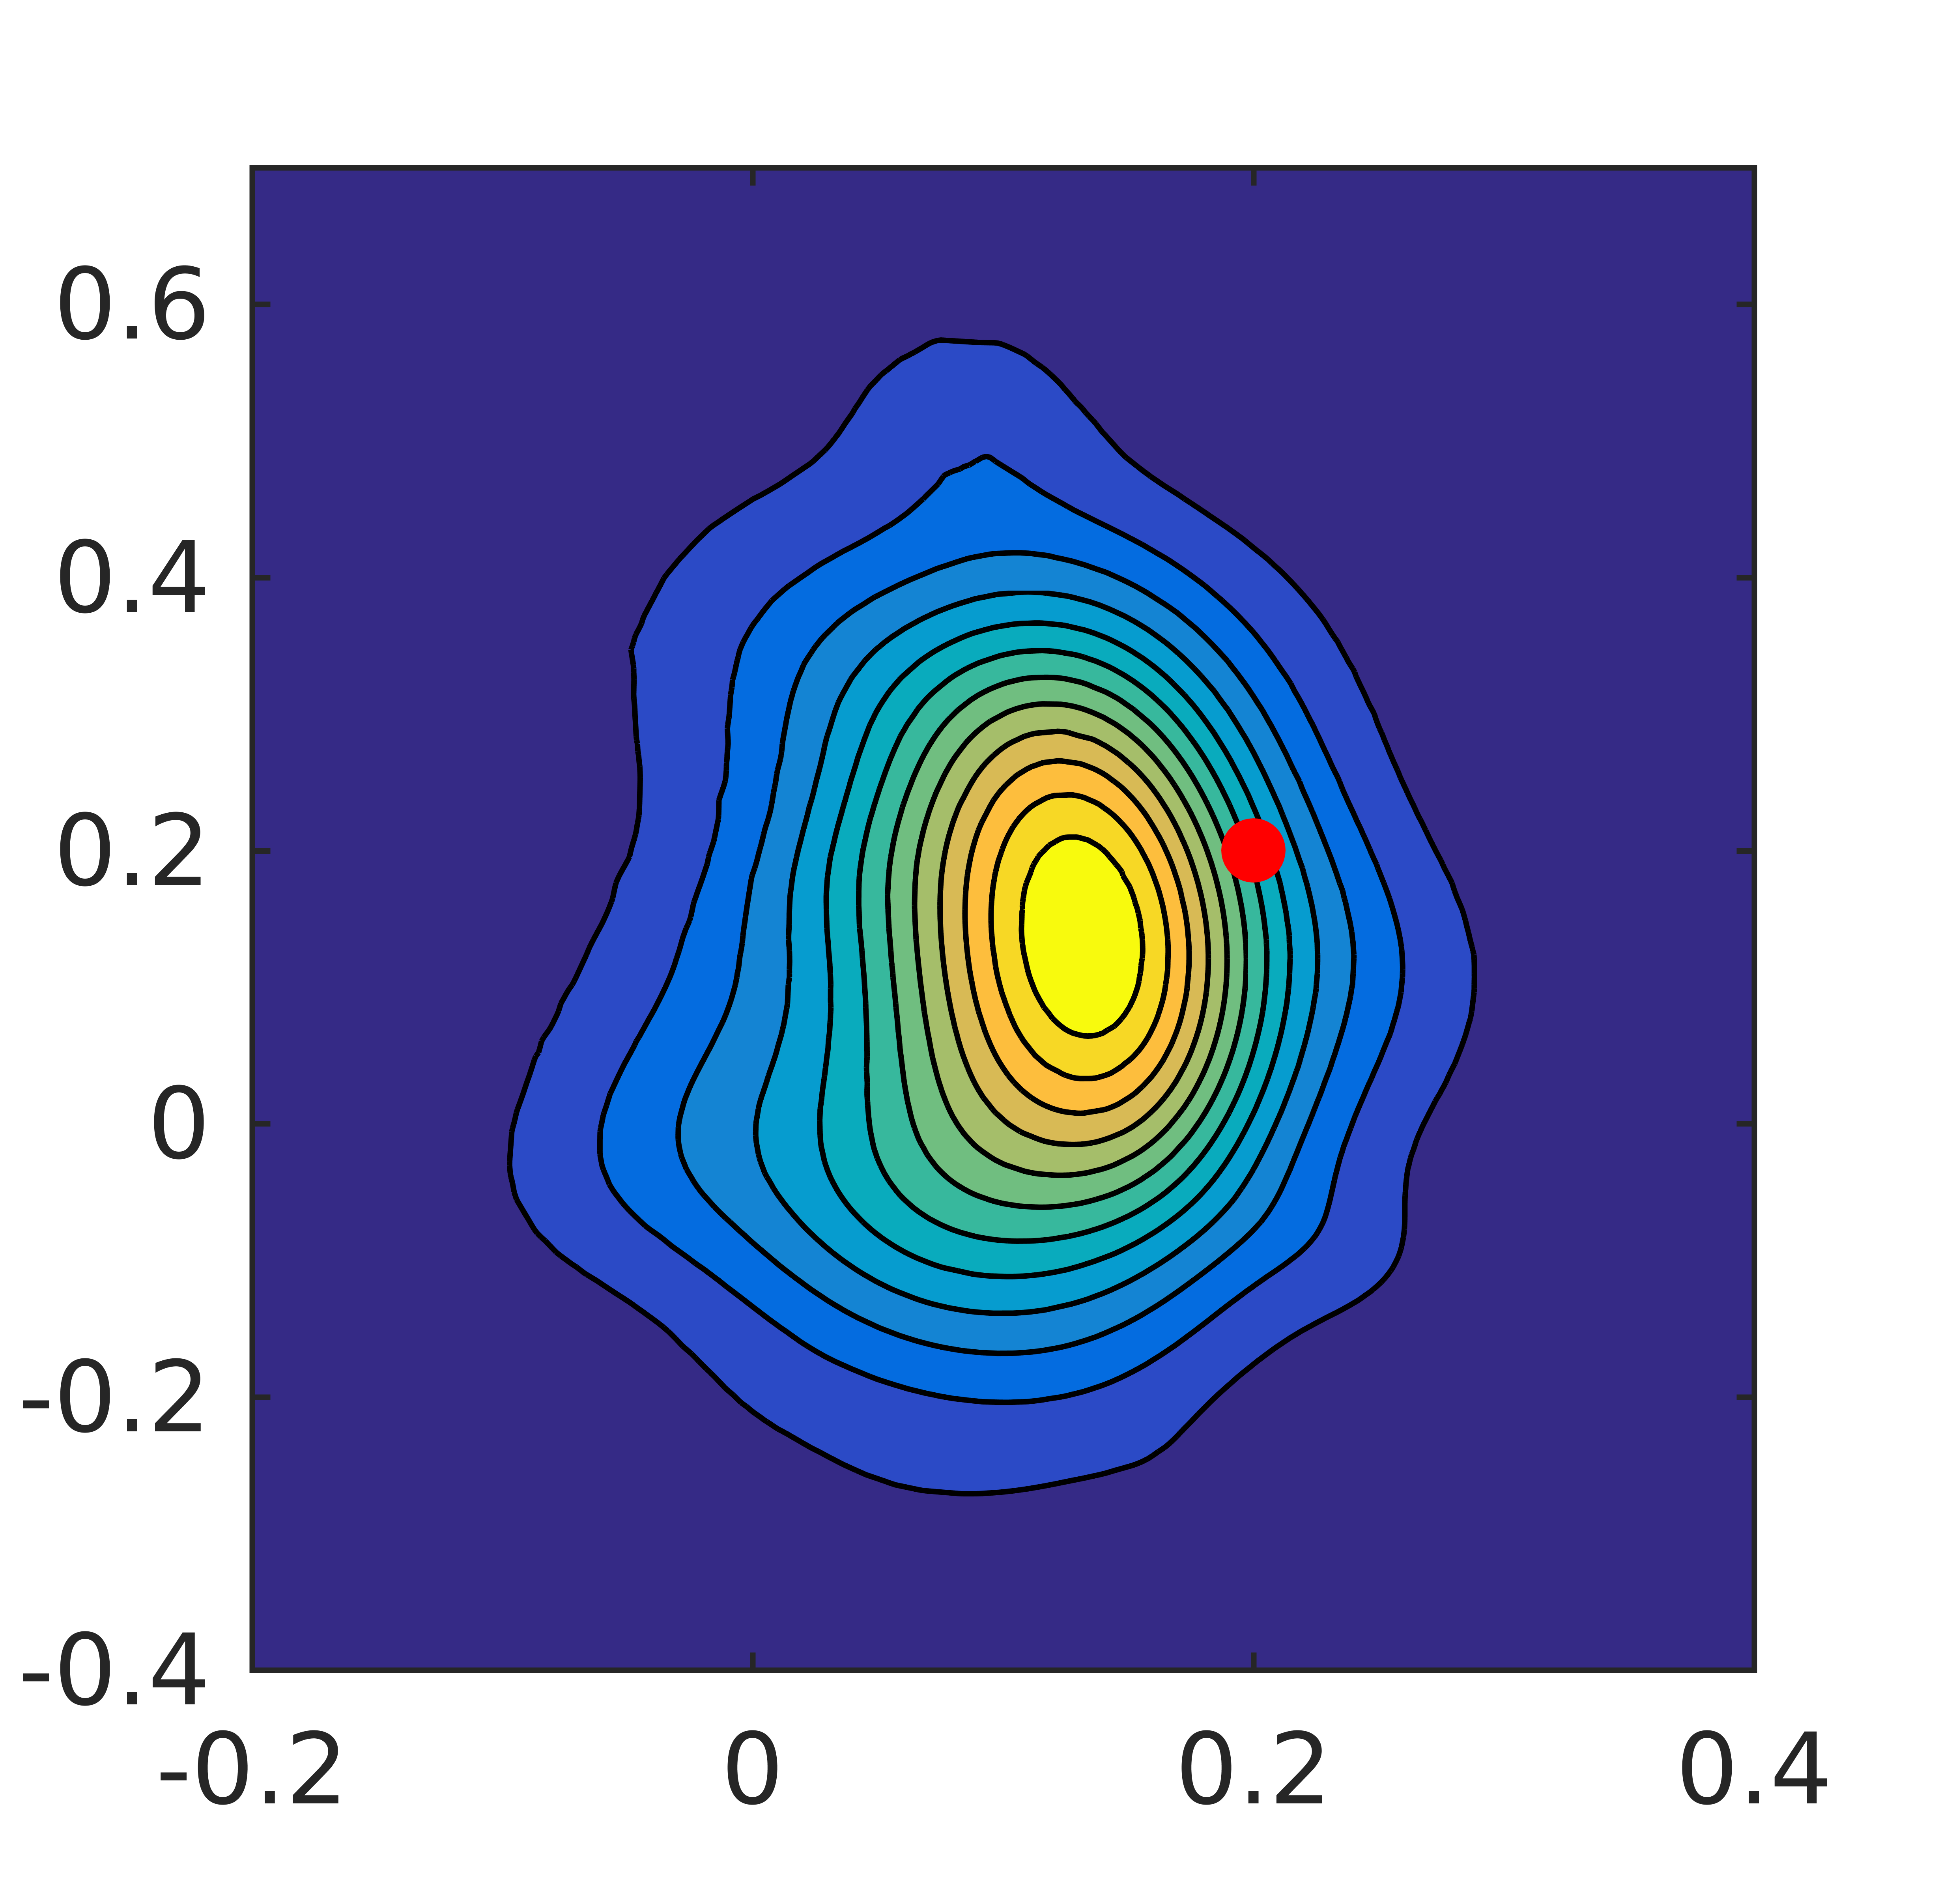
\includegraphics[]{MCMCFitznagAdd01.png} \\
			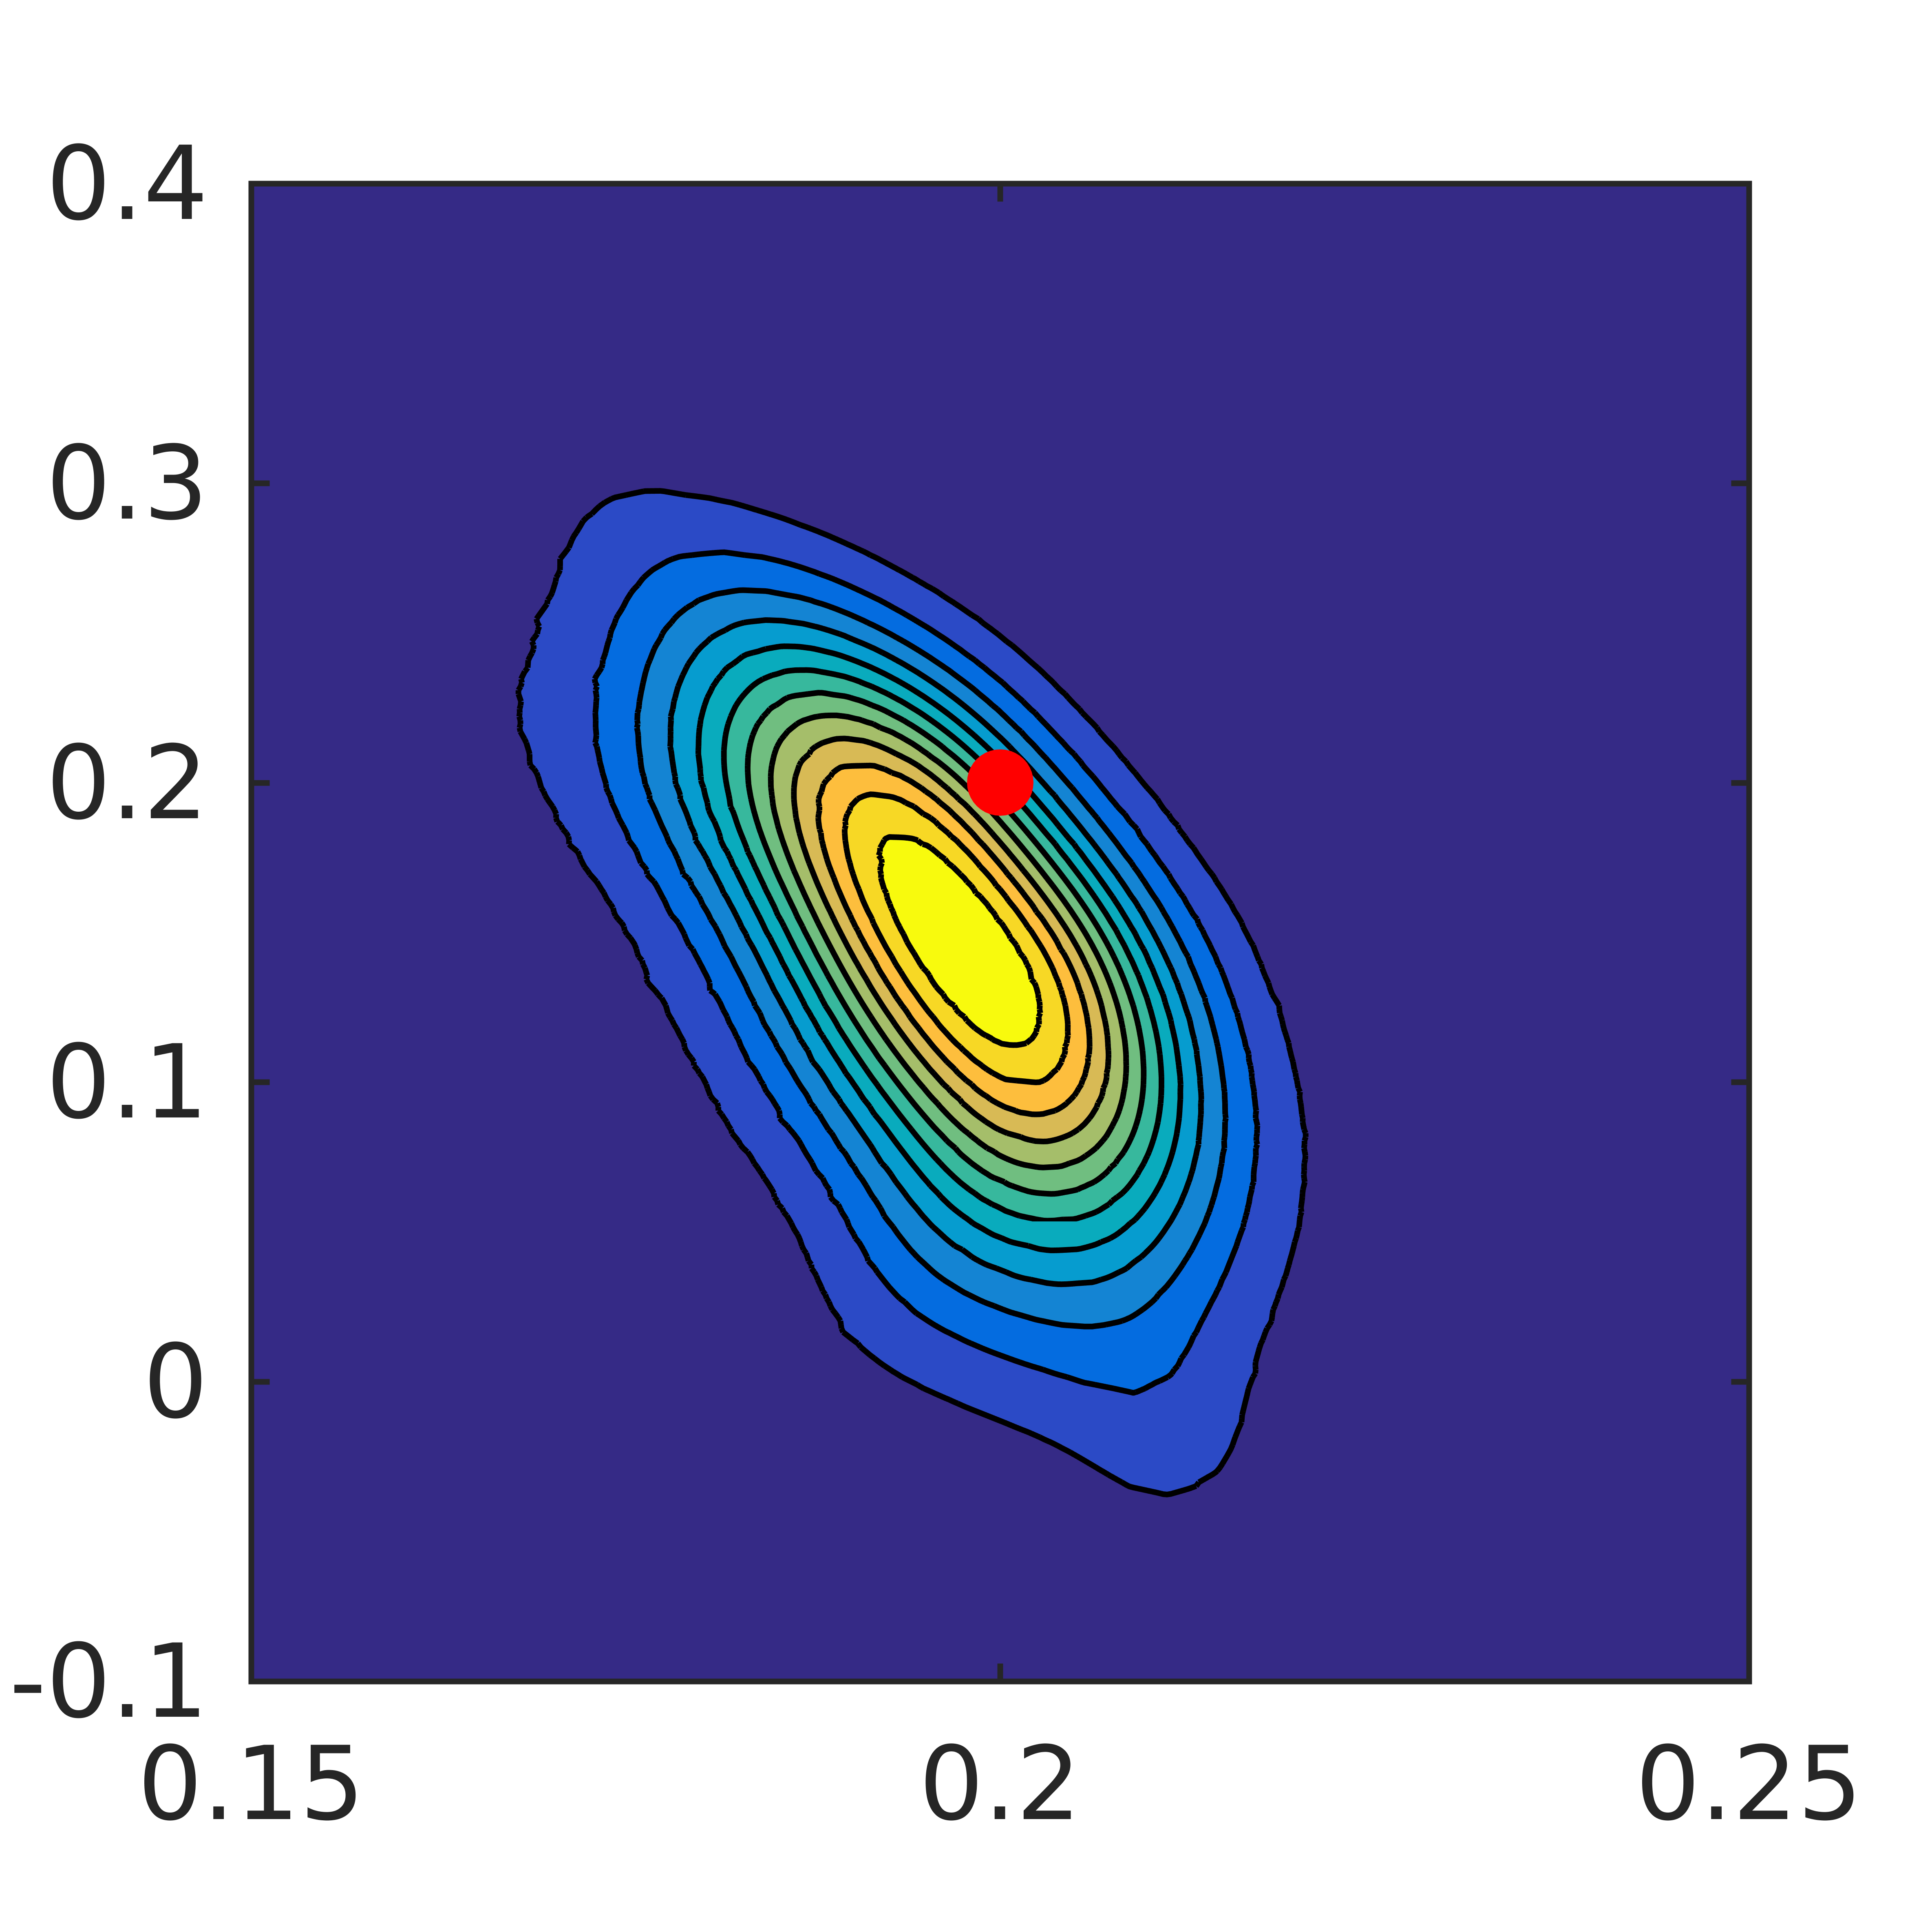
\includegraphics[]{MCMCFitznagStep001.png} & 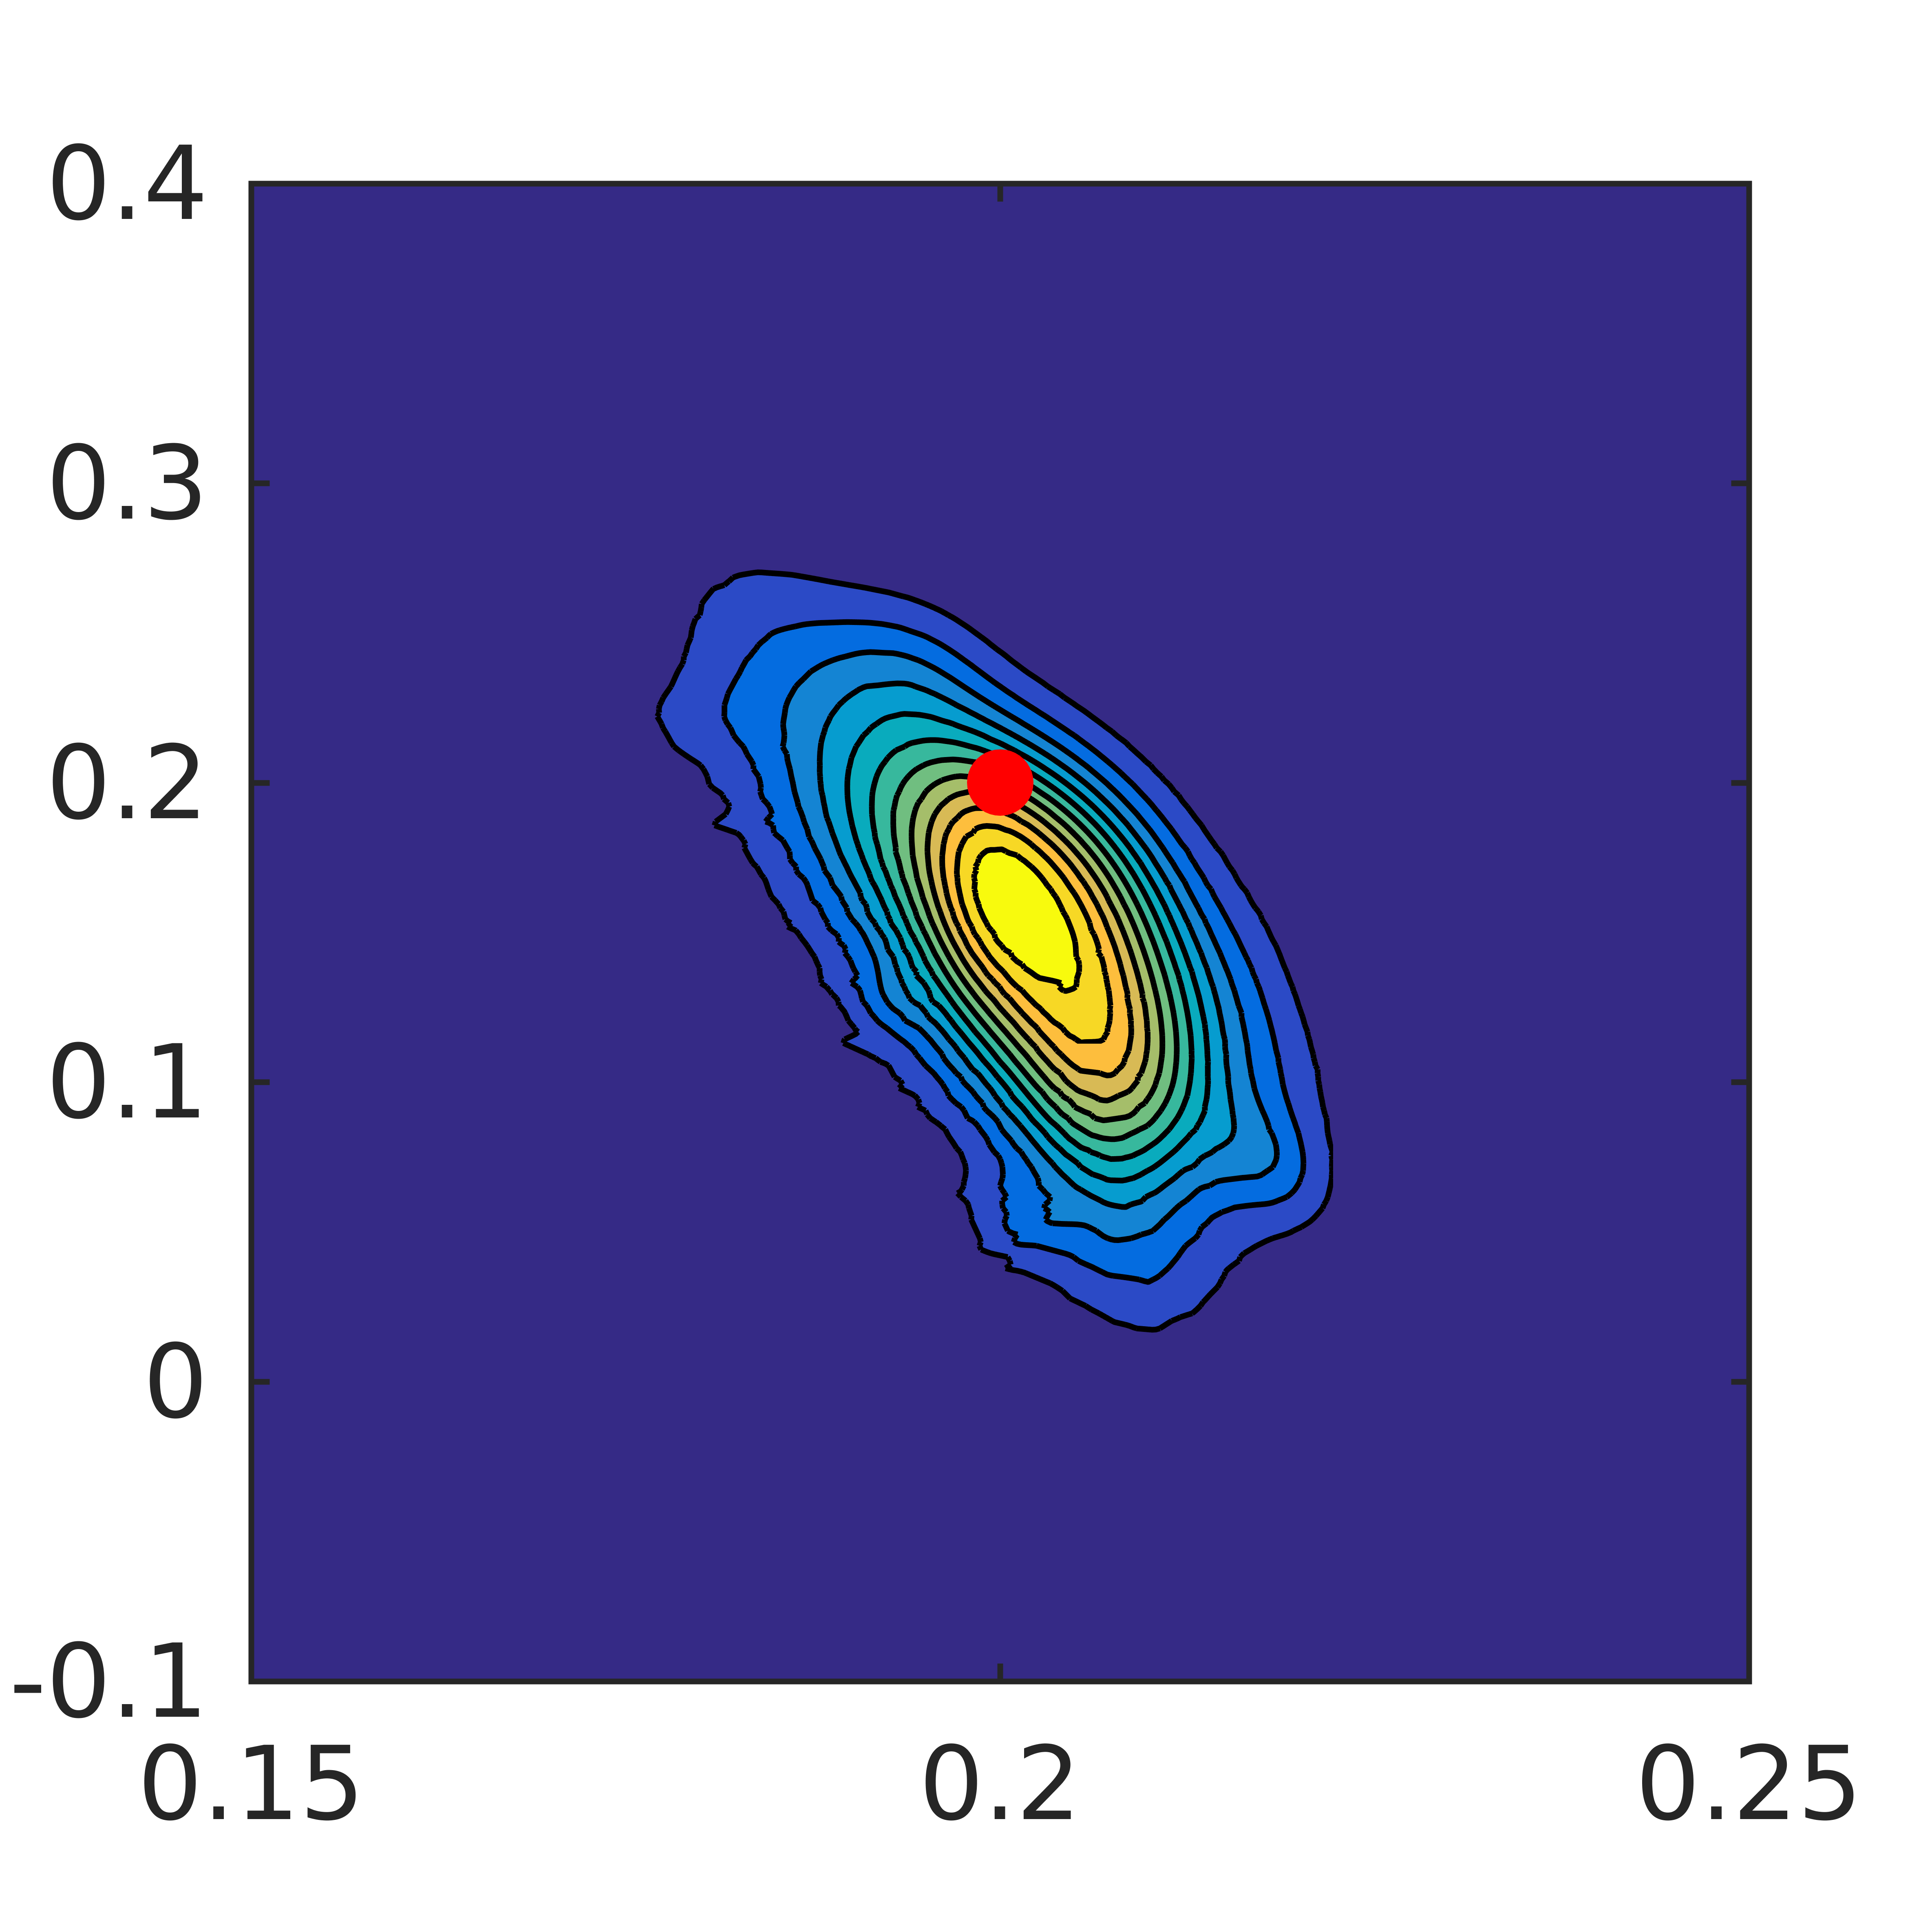
\includegraphics[]{MCMCFitznagAdd001.png} \\
		\end{tabular}
	\end{center}
	\caption{Posterior distribution for $(\theta_1, \theta_2)$ given by MCMC. Results given by \eqref{eq:ProbMethVarH} and \eqref{eq:ProbMethAddNoise} are on the left and right column respectively ($h = 0.1$ top, $h = 0.01$ bottom). The red dot indicates the true value of the parameter.}
	\label{fig:MCMC}
\end{figure}

We consider the FitzHug-Nagumo equations \eqref{eq:DistanceExactDet} and the problem of inferring the value of the parameter $\theta = (a, b, c)^T$. Inference is based on observations $\{y_i\}_{i=1}^{10}$ at times $\{t_i = i\}_{i=1}^{10}$, generated with a fine Runge-Kutta solver biased by Gaussian observational noise with variance $\Sigma = 0.01I$, where $I$ is the density matrix in $\R^{2\times 2}$. We generate samples of $\theta$ employing both the additive noise and the random time-stepping methods to approximate the likelihood in the frame of a noisy pseudo-marginal MCMC algorithm \cite{AnR09, MLR16}. In order to attain optimal acceptance ratio in the Markov chain, we employ the robust adaptive Metropolis algorithm (RAM) for tuning a Gaussian proposal distribution \cite{Vih12}. We choose a Gaussian prior distribution $\mathcal{Q}(\theta)$ centered in the true value $\bar \theta = (0.2, 0.2, 3.0)^T$ with unitary variance in the three components. We employ the explicit Euler method as the deterministic component with $h = 0.1$ and $h = 0.01$ for both \eqref{eq:ProbMethVarH} and \eqref{eq:ProbMethVarH}. In Figure \ref{fig:MCMC} we show the marginal posterior distribution of $(\theta_1, \theta_2)$ with $\theta_3$ fixed to its true value $\bar\theta_3$. It is possible to remark that the uncertainty due to numerical error is well accounted by both the probabilistic integrators.  


\bibliographystyle{siamplain}
\bibliography{anmc}

\end{document}